\documentclass[brazil,tf,epusp]{usp}  %Código de trabalho de formatura: tf
\usepackage[T1]{fontenc}  %Orienta a saída do texto a reproduzir caracteres especiais
\usepackage[utf8]{inputenc} %Permite que o usuário redija o documento utilizando caracteres especiais UTF-8

\usepackage{graphicx}  %Pacote de gerenciamento de figuras. Padrão para qualquer documento em LaTeX
\usepackage{helvet}  %Define Helvetica como fonte Sans Serif padrão
\usepackage{fancyvrb}  %Serve, por exemplo para aplicar estilos de texto individuais em trechos do texto
\usepackage{babel}  %Pacote de idioma
\usepackage{textcomp}  %Graças a esse pacote eu não preciso me preocupar com o símbolo °
%\usepackage{textgreek} %Define comandos para chamar letras gregas. Passei a usar o modo matemático pra isso.
%\usepackage{fixltx2e}  %Define \textsubscript{}, por exemplo.
\usepackage[font=normalsize]{subfig}  %Habilita utilização de subfiguras nos campos de figuras.
\usepackage{indentfirst}  %Faz a primeira linha após o chapter head ser indentada (vide definição de \thickline abaixo)
\usepackage{array}  %Graças a ele eu consigo editar elementos de tabela.
\usepackage{amssymb}  %Pacote com complementos do modo matemático.
\usepackage{amsmath}  %Pacote com complementos do modo matemático.
\usepackage[symbolgreek]{mathastext}  %Equações ficam na mesma fonte do texto graças a isso. http://jf.burnol.free.fr/v13/mathastext.pdf
%\usepackage{paralist}  %Possibilita a criação de listas (ambiente enumerate) "inline".
\usepackage[hang,flushmargin]{footmisc}  %Deixa a indentação do rodapé do jeito que eu quero (vide exemplos no texto).
\usepackage{enumerate}  %Formata rótulos de listas enumeradas

\usepackage{siunitx}  %Formatação grandezas sistema internacional
\sisetup{output-decimal-marker={,}}

\usepackage{multirow}  %Multi colunas e multi linhas em tabelas

\usepackage{chemformula}

\makeatletter
%%%Define linhas horizontais (\thickline) e verticais (') para tabelas
\newcommand{\thickhline}{
  \noalign {\ifnum 0=`}\fi \hrule height 1.5pt
  \futurelet \reserved@a \@xhline
}
\newcolumntype{'}{@{\hskip\tabcolsep\vrule width 1.5pt\hskip\tabcolsep}}
\makeatother

\begin{document}
\bibliographystyle{usp}

\autor{Paula Arantes Ribeiro}
\orientador{Prof. Dr. Hélio Goldenstein}
\coorientador{Dr. Arthur Seiji Nishikawa}
\titulo{Métodos de aprendizado de máquina para previsão de pontos críticos de equilíbrio em ligas multi-componente}

\departamento{ep-pmt}
% \programa{ep-metalurgica}
\renewcommand{\USPareadeconcentracaodata}{Engenharia de Materiais} %Define área de concentração Engenharia de Materiais
% Texto que vai na folha de rosto identificando a natureza do trabalho. Ao invés de utilizar o texto padrão, é possível redefini-lo usando o comando abaixo
\renewcommand{\USPcomentariodata}{\hyphenpenalty=10000%
Trabalho de formatura apresentado \`a Escola Polit\'ecnica da Universidade de
S\~ao Paulo para obtenção do t\'itulo de Engenheira}

% Agradecimentos do trabalho
%\agradecimentos{}
% ARRUMAR: escrever agradecimentos; folha errada.

% \textregistered{} não pode estar em resumo. Isso gera um erro na hora de compilar o texto
\resumo{
\setlength\parindent{0pt}
A proposta deste trabalho é avaliar diferentes algoritmos de aprendizado de máquina para prever temperaturas críticas de transformações de fases. Cálculos de termodinâmica computacional utilizando o software Thermo-Calc foram usados para gerar um banco de dados que representasse as composições químicas de aços de engenharia.
A partir dele, foram elaborados modelos de regressão linear multivariável e uma rede neural, cujas métricas e predições foram analisadas e comparadas entre si.
}
\palavrachave{Aço}
\palavrachave{Termodinâmica}
\palavrachave{Temperaturas críticas}
\palavrachave{Aprendizado de máquina}
\palavrachave{Regressão}
\palavrachave{Redes neurais}

% \resumole{}
% \palavrachavele{Steel}
% \palavrachavele{Thermodynamics}
% \palavrachavele{Critical temperatures}
% \palavrachavele{Machine learning}
% \palavrachavele{Regression}
% \palavrachavele{Neural Networks}

% Palavras chave na ficha catalográfica. 5 no máximo
\assunto{Aço}
\assunto{Termodinâmica}
\assunto{Aprendizado de máquina}
\assunto{Regressão}
\assunto{Redes neurais}

% Nomes na ficha catalográfica
\FCautorresumido{Ribeiro, P. A.}
\FCautorexpandido{Ribeiro, Paula Arantes}

\elementospretextuais{}  %Comando do USPTeX para criação dos elemenos pré-textuais do documento

\setlength\parindent{.85cm}  %Define em 0,85cm a identação da primeira linha do parágrafo.

\chapter{Introdução}

Aços têm diversas aplicações industriais e sua versatilidade está relacionada à variedade de propriedades que ele pode assumir. Além de sua composição química, processos de tratamento térmico controlam essas propriedades, que, por sua vez, estão relacionadas às temperaturas em que ocorrem as transformações de fases. Essas temperaturas também são chamadas de temperaturas críticas e, ao longo do tempo, foram desenvolvidos diversos métodos para determiná-las. Pode-se utilizar métodos experimentais, como a dilatometria, ou softwares de cálculos termodinâmicos, como o Thermo-Calc\textregistered{}, ou ainda equações empíricas.

Novos modelos estão em desenvolvimento e entre eles estão os algoritmos de aprendizado de máquina, cujo desempenho aumenta quanto maior for sua experiência em realizar alguma atividade. Apesar de os métodos atuais serem razoavelmente precisos e eficientes, eles demandam certo custo de equipamento, software ou capacitação humana. Assim, uma ferramenta de cálculo de fácil acesso e utilização permitiria melhor compreensão das temperaturas críticas para o tratamento térmico de aços.

\chapter{Objetivos}

O presente trabalho tem como objetivo a criação de um algoritmo de aprendizado de máquina para determinar as temperaturas críticas de transformação em aços de engenharia, utilizando a base de dados do software Thermo-Calc\textregistered{}, a fim de disponibilizar uma ferramenta de cálculo simples de se utilizar e aberta à comunidade científica.

\chapter{Revisão bibliográfica}

\section{Os componentes do aço}

Aços podem ser vistos como uma liga ferrosa com adições de carbono e outros elementos de liga, dentre os quais destacam-se o manganês, silício, cromo, níquel, entre outros \cite{Dossett2006}. São conhecidas inúmeras combinações de ligas de ferro e carbono que fornecem diferentes combinações de propriedades mecânicas, podendo apresentar altíssimas dureza e resistência (e.g., as novas gerações de aços avançados de alta resistência), ou serem maleáveis, como em aços de baixa liga. Tal mudança de propriedades está relacionada com as diferentes estruturas do ferro (fases) e combinações de morfologias que o aço pode assumir.

O ferro puro em estado sólido tem duas formas alotrópicas, ou seja, diferentes estruturas cristalinas que dependem da temperatura e pressão. A baixas temperaturas, o ferro assume a estrutura cúbica de corpo centrado (CCC) e é denominado $\alpha$-Fe, ou ferrita. Acima de 910~°C, a disposição atômica do ferro muda de CCC para cúbica de faces centradas (CFC), também chamada de $\gamma$-Fe, ou austenita. A estabilidade da austenita permanece até 1400~°C, quando volta a assumir uma estrutura CCC. Esta ferrita de alta temperatura é comumente chamada de $\delta$-Fe devido à diferente faixa de temperatura de ocorrência da fase $\alpha-Fe$. Alguns autores também diferenciam a fase $\beta$-Fe da fase $\alpha$-Fe, ambas de estrutura CCC, pelo fato de que para temperaturas superiores a 770~°C (temperatura de Curie) o $\alpha$-Fe perde suas propriedades ferromagnéticas e passa a ser paramagnético \cite{Totten2006}.

A partir da combinação dessas possíveis estruturas do ferro com outros elementos formam-se as ligas. Como o ferro é a base do aço e tem estruturas cristalinas limitadas, é a sua combinação com outros átomos que resulta em diferentes propriedades. O carbono possui baixa solubilidade na fase $\alpha$ (0,02\% em massa a 738~°C), mas é bastante solúvel na fase $\gamma$, pois a estrutura CFC permite a alocação de uma maior fração de átomos de carbono em seus interstícios.
% A presença do carbono diminui as temperaturas necessárias para que a liga de ferro sofra transformações de fases.

A porção de uma liga com estrutura e propriedades homogêneas é denominada fase. Em equilíbrio termodinâmico, as combinações entre o carbono e o ferro podem resultar em ferrita, austenita ou grafita, cujas relações com a temperatura e composição são mostradas no diagrama de equilíbrio da Figura \ref{fig:diagrama_fe-c}. Nessas condições, os constituintes do sistema Fe-C à temperatura ambiente seriam ferrita $\alpha$ e grafita.

\begin{figure}[ht!]
  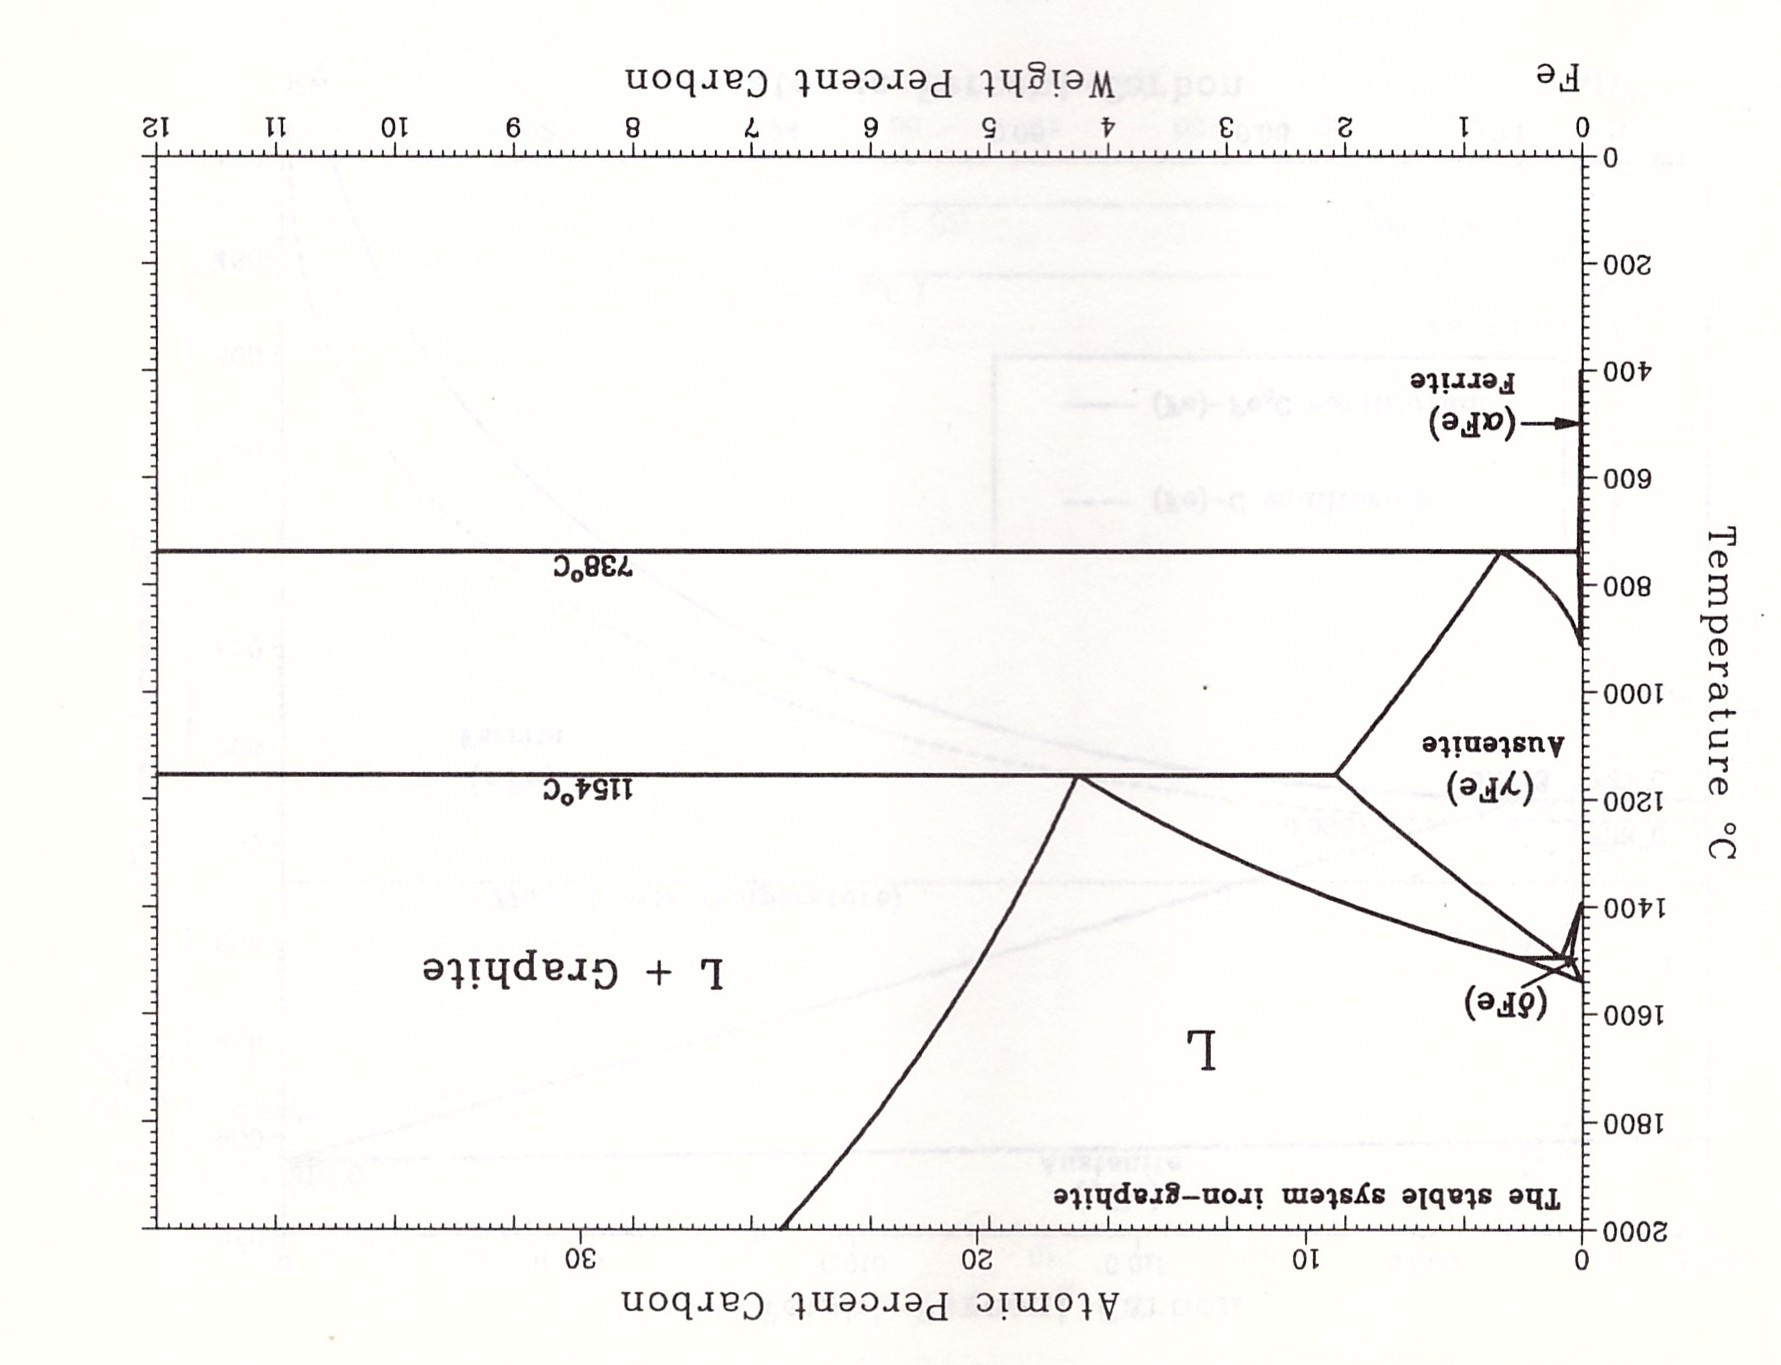
\includegraphics[width=.8\textwidth,angle=180]{img/Fe-C.jpg}
  \caption{Diagrama de equilíbrio ferro-carbono \cite{Massalski1996v1}}
  \label{fig:diagrama_fe-c}
\end{figure}

Entretanto, a condição de equilíbrio não é verificada para a maioria dos processos e, em vez de grafita, forma-se o carboneto de ferro \ch{Fe3C}, também chamado de cementita. A cementita é uma fase metaestável, mas sua formação é favorecida cineticamente em relação à grafita devido às elevadas taxas de resfriamento aplicadas ao aço durante seu processamento.
% uma vez que a solidificação e resfriamento do aço são muito rápidos.
% , que apesar de ser uma fase metaestável pode ser considerada estável, pois o coeficiente de difusão do carbono no ferro é muito baixo (\SI{2,9e-19}{cm^2/s}).
Para essas condições, o diagrama de fase, que é então chamado de diagrama de equilíbrio metaestável, é dado pela Figura \ref{fig:diagrama_fe-c_meta}.

\begin{figure}[ht!]
  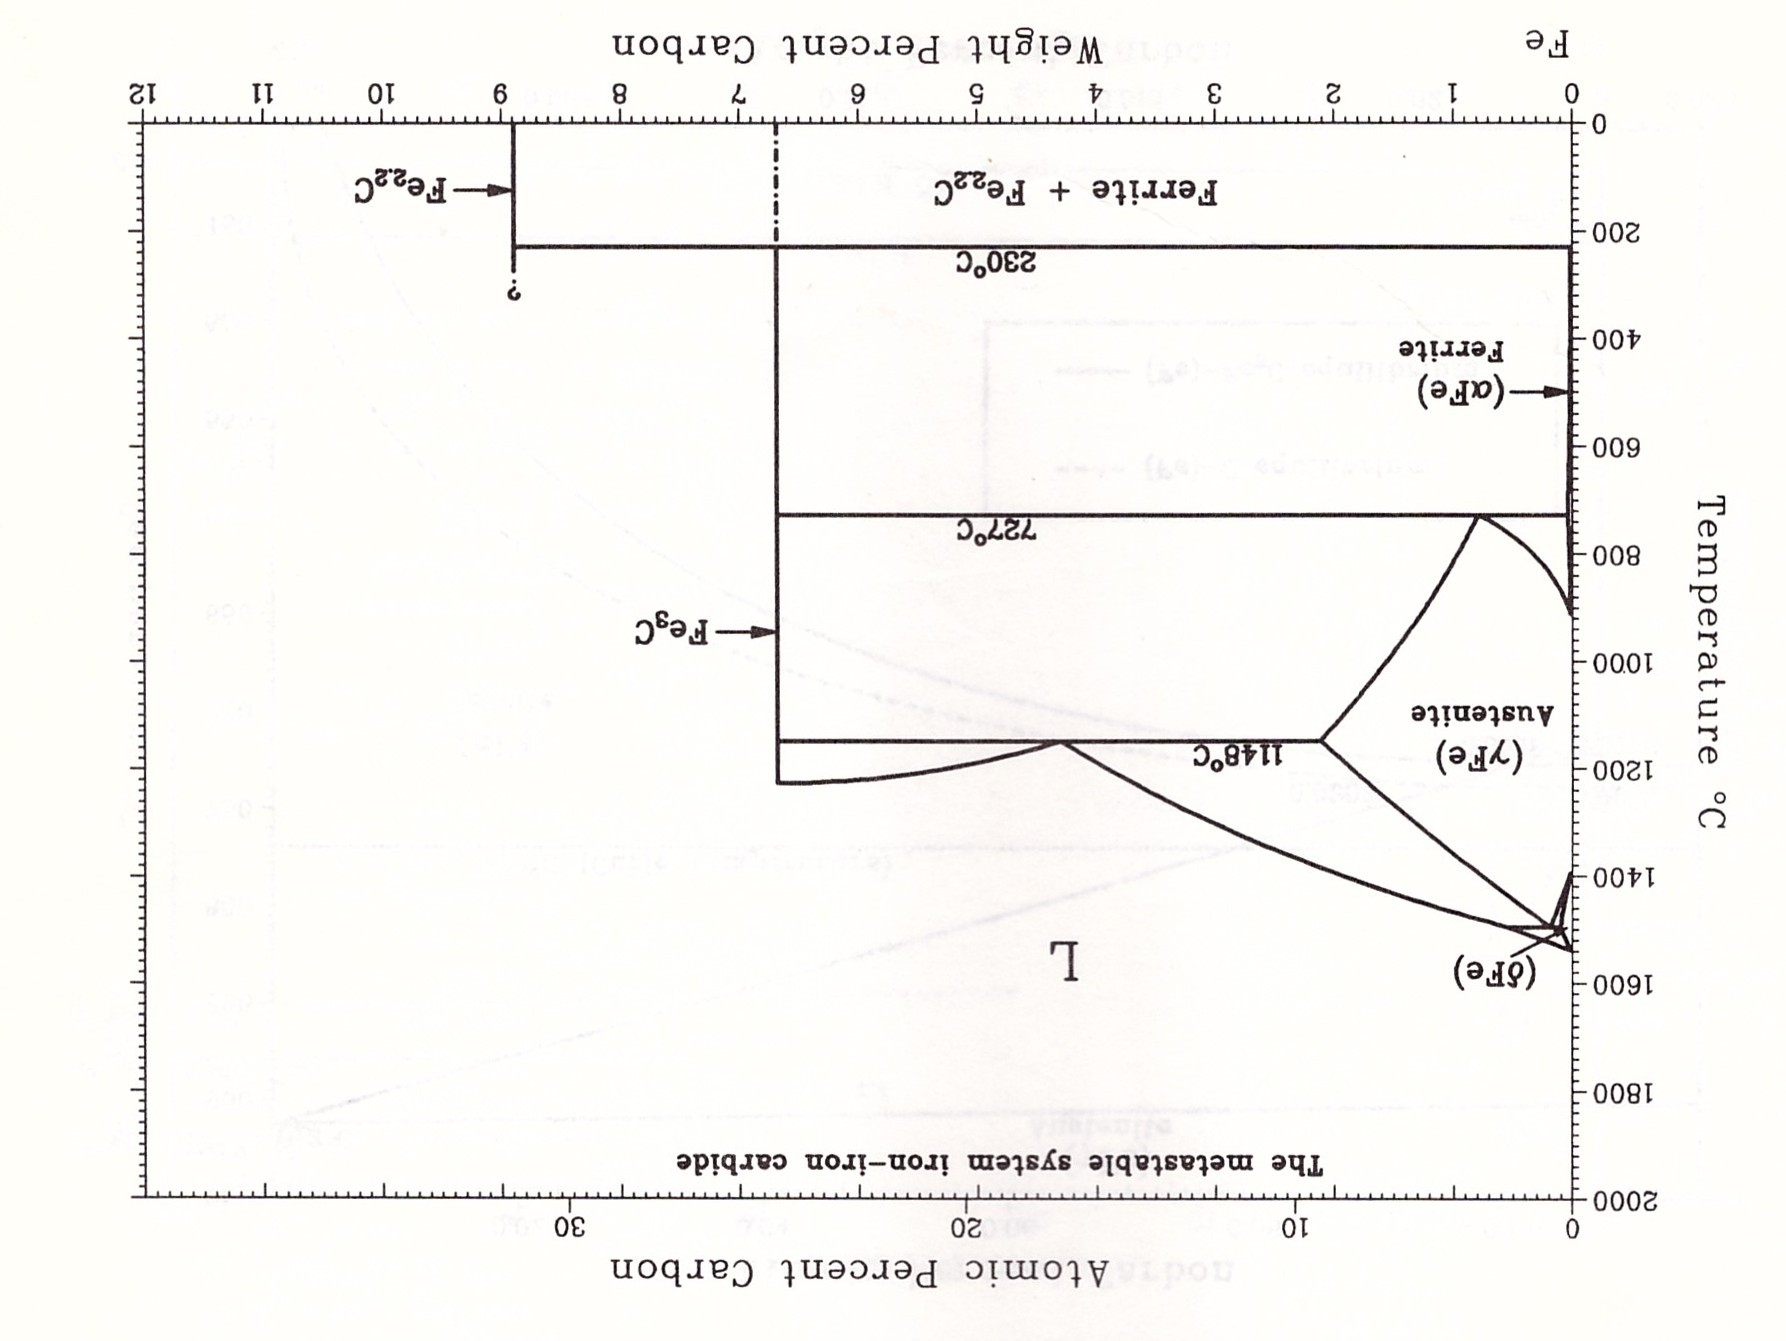
\includegraphics[width=.8\textwidth,angle=180]{img/Fe-C_meta.jpg}
  \caption{Diagrama de fases metaestável ferro-carbono \cite{Massalski1996v1}}
  \label{fig:diagrama_fe-c_meta}
\end{figure}

Um ponto importante do diagrama mostrado na Figura \ref{fig:diagrama_fe-c_meta} é o ponto eutetóide, no qual coexistem em equilíbrio as fases $\alpha$, $\gamma$ e \ch{Fe3C}. Para um sistema apenas ferro e carbono, o teor de carbono correspondente a esta fase é aproximadamente 0,8\% C em massa. Ligas com teores de carbono inferiores a esta composição são denominadas hipoeutetóides e, ligas com teores de carbono superiores à do ponto eutetóide são chamadas de hipereutetóides.

\section{Decomposição da Austenita}

\textbf{PENSANDO BEM, ACHO QUE VOCÊ NÃO PRECISA DESSA SEÇÃO. SEU TRABALHO É SOBRE TRANSFORMAÇÕES NO EQUILÍBRIO METAESTÁVEL}

Para uma liga Fe-C resfriada lentamente até a temperatura ambiente, o teor de carbono é fator determinante na natureza e proporção da fases formadas. Por sua vez, a taxa de resfriamento controla a formação de constituintes metaestáveis. Essa formação de constituintes a partir da austenita pode ocorrer por difusão, cisalhamento ou uma mistura dos dois mecanismos \cite{Honeycombe1982}.

No caso da ferrita, o resfriamento lento resulta em grãos equiaxiais preferencialmente no contorno de grão austenítico, enquanto um resfriamento rápido gera grãos em forma de agulhas, também conhecidos como ferrita acicular, nucleados no contorno e no interior do grão austenítico \cite{Silva2010} %{Krauss1997}apud{Silva2010} ARRUMAR.
A cementita segue o mesmo comportamento morfológico e ambas ocorrem sob mecanismo exclusivo de difusão \cite{Honeycombe1982}.

Para um aço de composição eutetóide, o resfriamento lento produz perlita, uma microestrutura característica que na realidade é uma mistura de austenita e cementita, na forma de lamelas. A ferrita é menos compacta por ter estrutura CCC e, consequentemente, apresenta insterstícios tetraédricos menores. Assim, à medida que o resfriamento ocorre, o carbono da austenita é rejeitado pela ferrita em formação, dando origem à cementita, fase rica em carbono \cite{Silva2010}.

Já um aço carbono resfriado bruscamente produz a martensita, uma estrutura que mantém o carbono em solução sólida da austenita. Diferente da formação de ferrita e perlita, esse processo não é controlado pela difusão devido à sua condição de resfriamento, mas sim por uma distorção na rede. Dessa forma, é um constituinte de mesma composição da austenita. Ela é característica pela sua microestrutura em ripas e alta dureza \cite{Honeycombe1982}.

Já a bainita é um constituinte intermediário, pois reúne o rearranjo de rede da martensita à redistribuição de carbono e precipitação de carboneto da perlita \cite{Totten2006}. Sua natureza se modifica com a diminuição da temperatura de transformação, sendo classificada em bainita superior e inferior. A morfologia da bainita superior contem ferrita na forma de ripas, de concentração de carbono muito inferior à da austenita mãe; já a cementita depende do teor de carbono, podendo assumir a forma de partículas isoladas ou mesmo não precipitar, permanecendo na forma de austenita retida. Já a bainita inferior é mais acicular e tem lamelas mais individualizadas \cite{Honeycombe1982}.

\section{O software Thermo-Calc\textregistered{}}
\textit{(Ainda será escrito)}

\section{Temperaturas cr\'iticas de aços}

Le Chatelier foi o primeiro a atribuir a letra ``A'' para as temperaturas críticas de transformação, devido à palavra \textit{Arrêt}, que representa a parada na temperatura durante a transformação de fase \cite{Silva2010}. Para exemplificar essas temperaturas críticas em aços, são mostrados a seguir gráficos obtidos por simulações de termodinâmica computacional determinados utilizando o software Thermo-Calc\textregistered{} correspondentes a uma liga Fe-1\%Mn-C.

A Figura \ref{fig:fe-1mn-C_isopleth} corresponde à isopleta do carbono para o teor de 1\% em massa de Mn. As linhas tracejas na vertical representam três ligas com teores de carbono também fixos. A primeira linha vertical tracejada da Figura \ref{fig:fe-1mn-C_isopleth} representa um aço hipoeutetóide e o gráfico da fração molar das fases em função da temperatura é apresentado na Figura \ref{fig:fe-1mn-c}a. Um aço com essa composição, mediante aquecimento, mantém as fases $\alpha$ e \ch{Fe3C} estáveis até a temperatura A1 ser atingida, na qual a fase $\alpha$ começa a se decompor em $\gamma$. No gráfico da Figura \ref{fig:fe-1mn-c}a, essa temperatura pode ser notada pela primeira mudança de inclinação da curva da austenita. O aço permanece no campo trifásico ($\alpha$ + $\gamma$ + \ch{Fe3C}) até a temperatura A1' ser atingida, quando toda a fase \ch{Fe3C} é consumida. Para temperaturas crescentes, a fase $\alpha$ se transforma em $\gamma$ até a temperatura A3 ser atingida, na qual tem-se 100\% de fase $\gamma$.

\begin{figure}[ht!]
  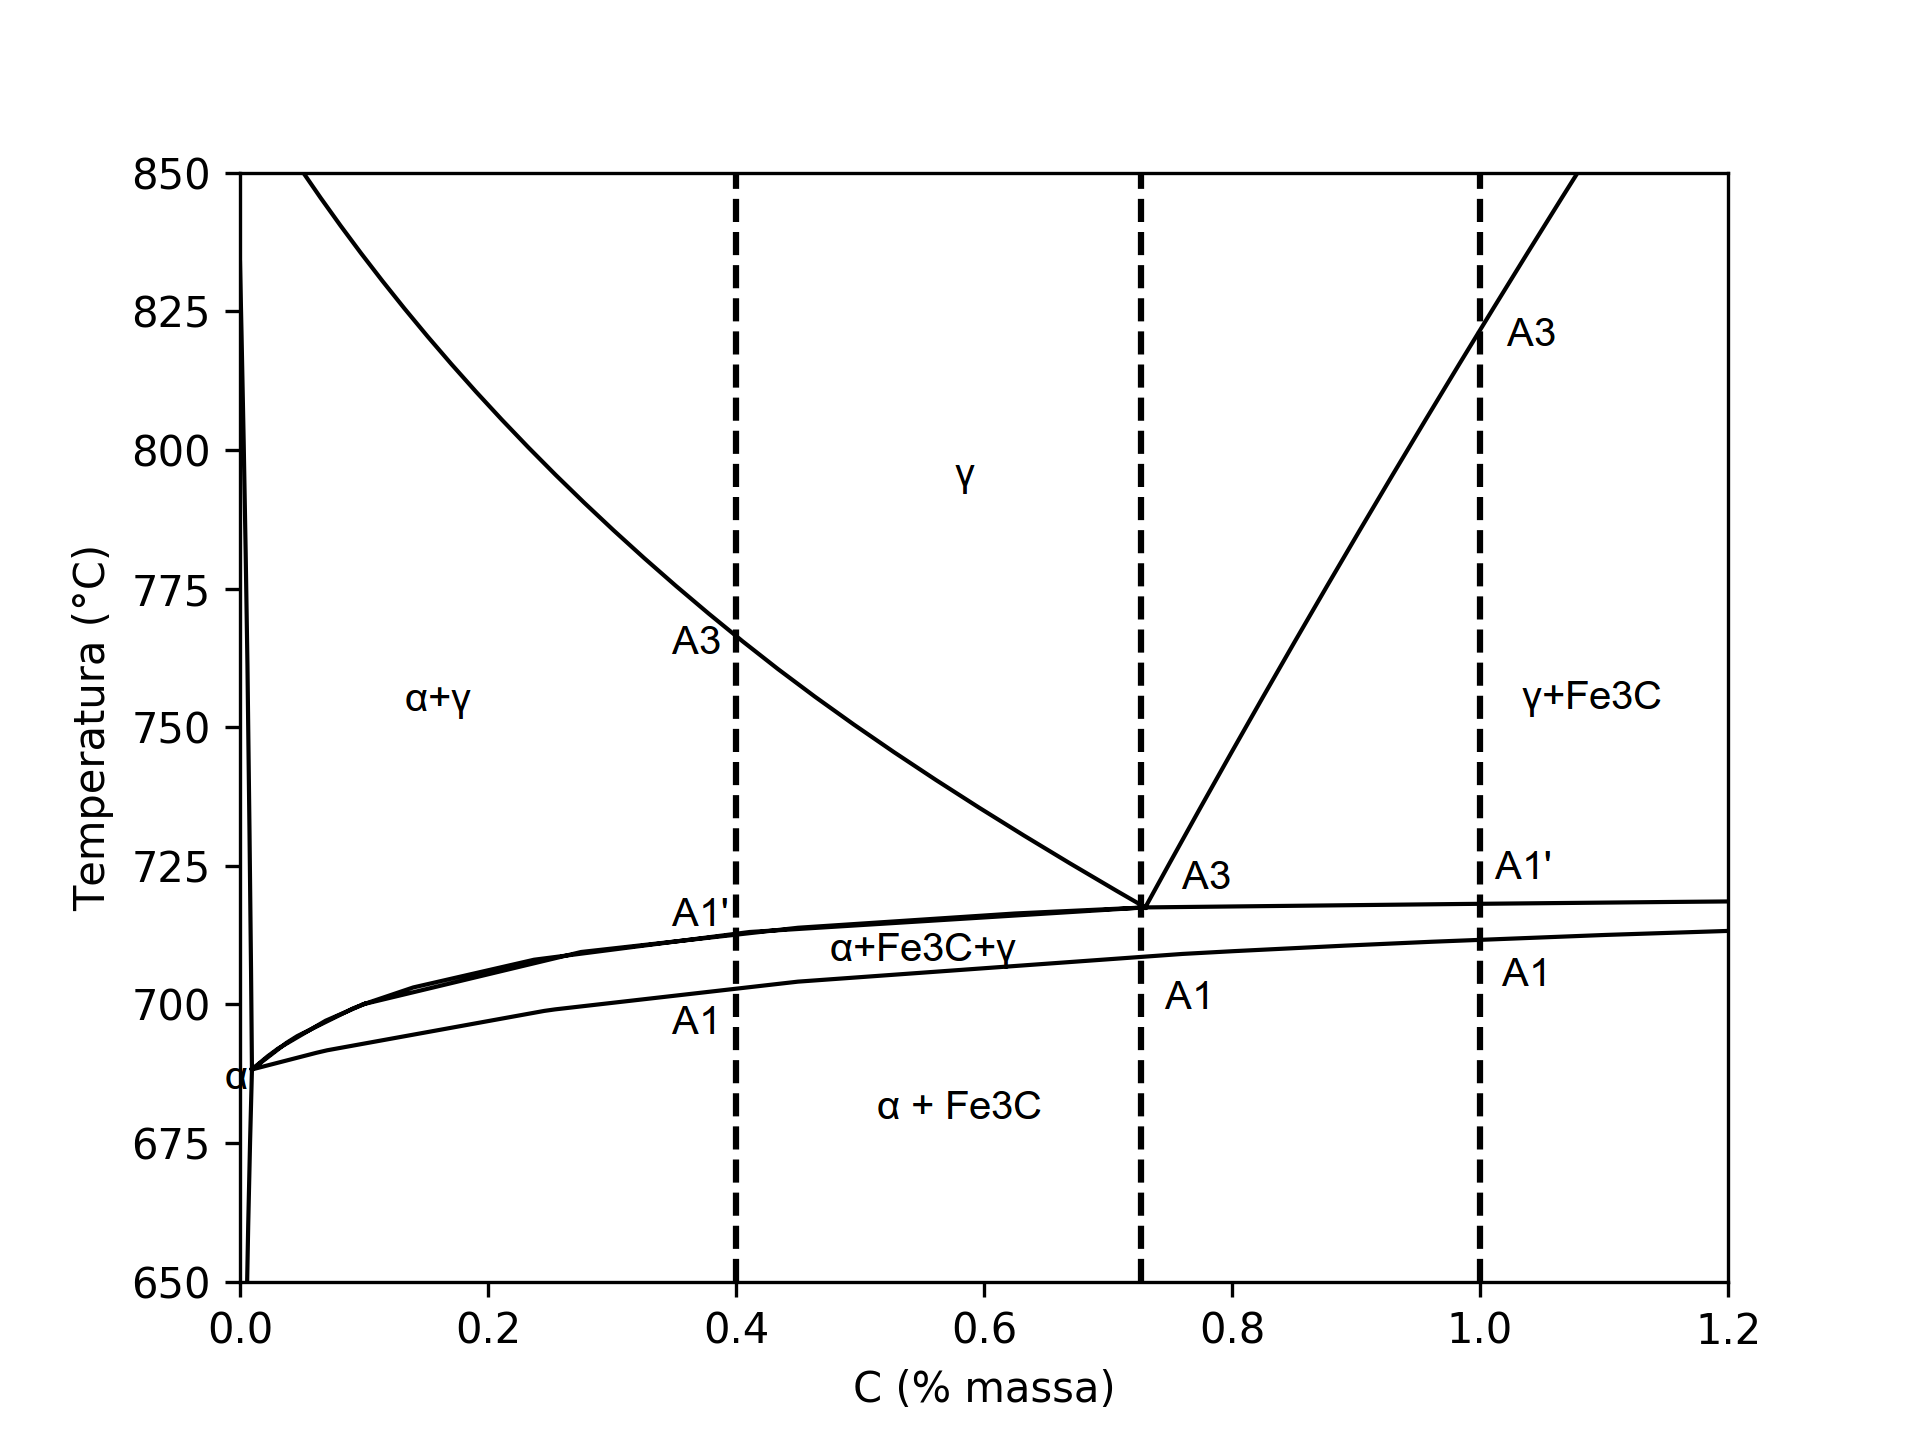
\includegraphics[width=.9\textwidth]{img/Fe-1Mn-C_isopleth_edited.png}
  \caption{Diagrama de fases Fe-C para aço 1\% Mn, em massa}
  \label{fig:fe-1mn-C_isopleth}
\end{figure}

\begin{figure}[ht!]
  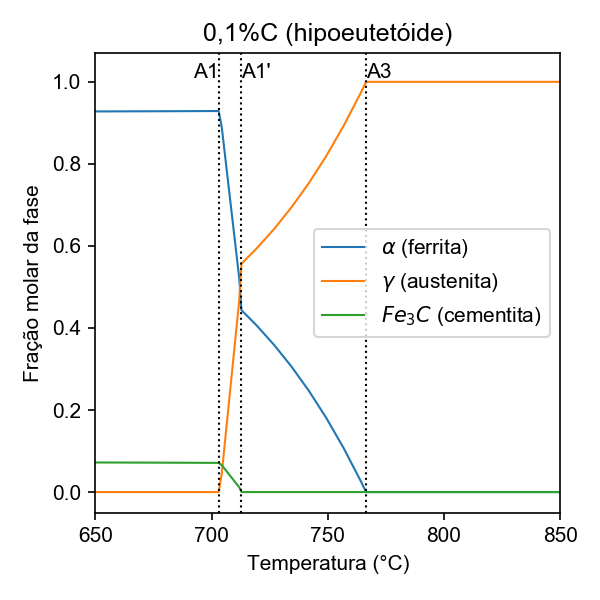
\includegraphics[width=.5\textwidth]{img/FE-1MN-04C.png}\hfill
  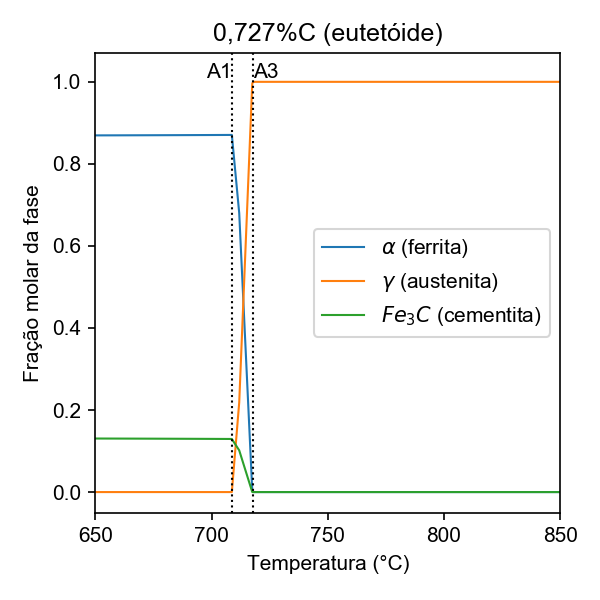
\includegraphics[width=.5\textwidth]{img/FE-1MN-0727C.png}\\
  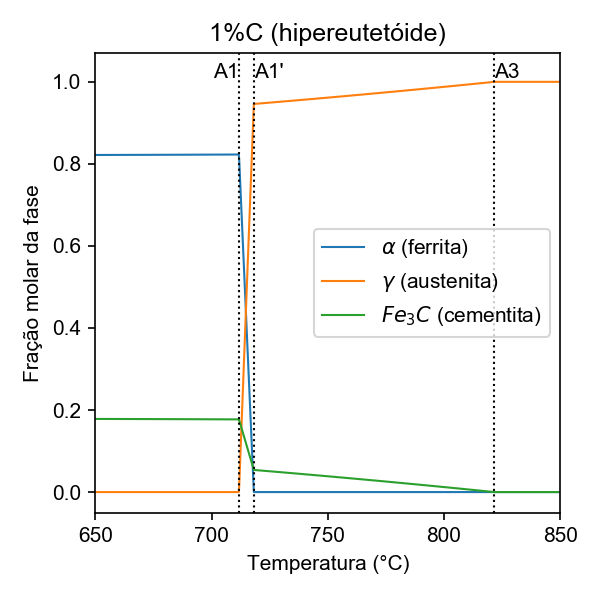
\includegraphics[width=.5\textwidth]{img/FE-1MN-1C.png}
  \caption{Fração molar de fase versus Temperatura para aço 1\%C 1\% Mn, em massa}
  \label{fig:fe-1mn-c}
\end{figure}

Um aço eutetóide, correspondente à segunda linha vertical da Figura \ref{fig:fe-1mn-C_isopleth} e ao gráfico da Figura \ref{fig:fe-1mn-c}b, segue o mesmo raciocínio. A diferença é que não há um campo trifásico e, portanto, não há mais uma temperatura A1' definida.

Já para um aço hipereutetóide, terceira linha vertical na Figura \ref{fig:fe-1mn-C_isopleth} e gráfico da Figura \ref{fig:fe-1mn-c}c, a diferença é que o segundo campo bifásico é constituído por $\gamma$ e \ch{Fe3C}, até atingir o ponto em que toda a fase \ch{Fe3C} se transforma em $\gamma$. Algumas referências, como \citaremsentenca{Digges1960}, fazem distinção para a temperatura A3 de aços hipereutetóides, chamando-a de Acm, devido à diferença de campos bifásicos. No presente trabalho, ambas serão chamadas de A3, por corresponderem à menor temperatura em que a fração de austenita é 100\%.

Em resumo, pode-se dizer que a temperatura A1 corresponde à máxima temperatura em que a fração de austenita é zero, enquanto a A3 é a mínima temperatura cuja fração de austenita é 100\% e A1' é o limite superior do campo intercrítico de três fases \cite{Honeycombe1982}.

É possível ainda diferenciar a temperatura crítica no resfriamento da de aquecimento, utilizando respectivamente as letras ``r'' e ``e''. Sob aquecimento e resfriamento lentos (ou seja, sob condições de equilíbrio) elas devem ser iguais. Na prática, as taxas de resfriamento ou aquecimento aplicadas deslocam as temperaturas Ae1 de Ar1 e Ae3 de Ar3 do equilíbrio, devido às cinéticas de formação e dissolução das fases. A faixa de temperatura entre A1 e A3 é chamada de intervalo crítico ou de transformação \cite{Digges1960}.

\section{Tratamento térmico de aços}

A importância da determinação das temperaturas críticas está diretamente relacionada à aplicação de tratamentos térmicos a aços. A obtenção das propriedades ideais de um aço está relacionada tanto com sua composição química quanto com os processos de tratamento térmico aos quais ele é submetido \cite{Totten2006}. Tratamentos térmicos podem ser utilizados para aumentar ou diminuir a ductilidade, dureza, tensão de escoamento ou tenacidade, otimizando essas propriedades para a finalidade do material \cite{Silva2010}.

A austenitização é a etapa que precede um tratamento térmico e consiste em aquecer o aço a uma temperatura em que haja formação da austenita. Esta pode ser parcial, quando se encontra na faixa de transformação (ou seja, entre as temperaturas A1 e A3), ou total, quando está acima do intervalo de transformação (acima da temperatura A3) \cite{ASM1991}.

%RECOZIMENTO
A partir do aço na forma de austenita, é possível fazer o recozimento, ou seja, o resfriamento lento para reduzir tensões, diminuir dureza, melhorar a usinabilidade ou ajustar o tamanho do grão, reduzindo assim influências de tratamentos térmicos ou mecânicos anteriores. Para aços hipoeutetóides a temperatura é de aproximadamente \SI{50}{\celsius} acima de A3, enquanto para hipereutetóides é de \SI{50}{\celsius} acima de A1, não podendo ultrapassar A3 pois em um resfriamento posterior formaria cementita nos contornos de grão da austenita, fragilizando a peça tratada. Quando se deseja uma estrutura perlítica, prefere-se temperaturas de austenitização mais altas, e mais baixas para estrutura esferoidizada. Para ambos os casos, quanto mais próxima de A1 for a temperatura de transformação da austenita, mais grosseira será a estrutura .

%NORMALIZAÇÃO
Outro tipo de tratamento térmico é a normalização, que após austenitização resfria lentamente o aço ao ar parado ou agitado, sendo recomendada para homogeneizar a estrutura após forjamento ou antes de outros processos, como têmpera ou revenimento. Em aços hipoeutetóides, causa um espaçamento entre as lamelas da perlita, tornando-a mais fina. A dureza e a resistência mecânica ficam mais elevadas e a dutilidade mais baixa. Para hipereutetóides, distribui-se melhor os carbonetos, pois a temperatura de austenitização ocorre acima de A3.

%TÊMPERA
Um terceiro tipo de processo muito importante é a têmpera, que consiste em resfriar o aço austenitizado rapidamente a fim de obter a estrutura metaestável martensítica. O teor de carbono aumenta a dureza da martensita e diminui a temperatura necessária para que o processo ocorra. Essa temperatura depende não só da composição do aço, mas também da taxa de resfriamento, e é chamada de Ms. Por depender de fatores cinéticos, essa temperatura crítica não será o foco do presente trabalho.

%REVENIMENTO
A formação de martensita aumenta a dureza do aço, entretanto o torna mais frágil. Para  melhorar a resistência mecânica e tenacidade do material temperado, realiza-se o revenimento da martensita, aquecendo o aço até temperatura inferior à de austenitização, mantendo-a até que as propriedades desejadas sejam alcançadas \cite{Silva2010}. Como a martensita é uma solução supersaturada de carbono, durante o revenimento o ferro o rejeita na forma de carbonetos em uma matriz de ferro $\alpha$ \cite{Honeycombe1982}.

\section{Efeito dos elementos de liga nas temperaturas críticas e tratamento térmico}
%INSERIR DIAGRAMAS BINÁRIOS
Os elementos de liga são adicionados ao aço para modificar as fases ou constituintes em equilíbrio, bem como alterar a maneira como essas fases se formam \cite{Silva2010}.

% Quanto maior o teor de carbono, maior a temperabilidade do aço. Entretanto, esse também fica mais suscetível a trincas durante a têmpera. Assim, a adição de elementos de liga tem como um de seus objetivos manter a alta temperabilidade do aço com baixa suscetibilidade a trincas, através da transformação da austenita em menor velocidade \cite{Souza1989}.

Os elementos de liga podem ser classificados de acordo com sua influência no campo austenítico, que por sua vez está relacionada à estrutura eletrônica dos elementos. São eles:

\begin{itemize}
  \item Classe 1: elementos de domínio $\gamma$ aberto (Figura \ref{fig:elem-liga}a), podendo até mesmo eliminar completamente a fase $\alpha$ em concentrações suficientemente altas. Assim, as transformações $\gamma \rightarrow  \alpha$ ocorrem a temperaturas menores, ou seja, A3 diminui e pode haver casos em que não há a temperatura A1. Fazem parte desse grupo: Níquel, Manganês, Cobalto, Rutênio, Ródio, Paládio, Ósmio, Irídio e Platina.

  \item Classe 2: elementos de domínio $\gamma$ expandido (Figura \ref{fig:elem-liga}b) até a formação de um composto de ferro. Essa expansão é responsável por formar solução sólida homogênea, sendo muito importante para o tratamento térmico dos aços. Pertencem a esse grupo o Carbono e o Nitrogênio, que diminuem o valor de A3.

  \item Classe 3: domínio $\gamma$ fechado (Figura \ref{fig:elem-liga}c), elementos que favorecem a expansão do domínio $\alpha$, que circunda o campo austenítico, formando uma região chamada de ilha gama ou $\gamma$-loop. Estes aumentam A1 e pode haver casos em que A3 não existe. Essas ligas não podem passar por tratamento térmico de arrefecimento através da transformação $\gamma \rightarrow \alpha$. Fazem parte desse grupo: Silício, Alumínio, Berílio, Fósforo e elementos fortemente formadores de carboneto, como Titânio, Vanádio, Molibdênio e Cromo.

  \item Classe 4: domínio $\gamma$ contraído mas há formação de compostos de ferro (Figura \ref{fig:elem-liga}d). Os elementos Boro, Enxofre, Tântalo, Nióbio, Zircônio estão nessa categoria \cite{Honeycombe1982} \cite{Silva2010}.
\end{itemize}

% A Figura \ref{fig:elem-liga} mostra a influência dos elementos de liga no campo austenítico em diagramas binários de ferro.

\begin{figure}[ht!]
  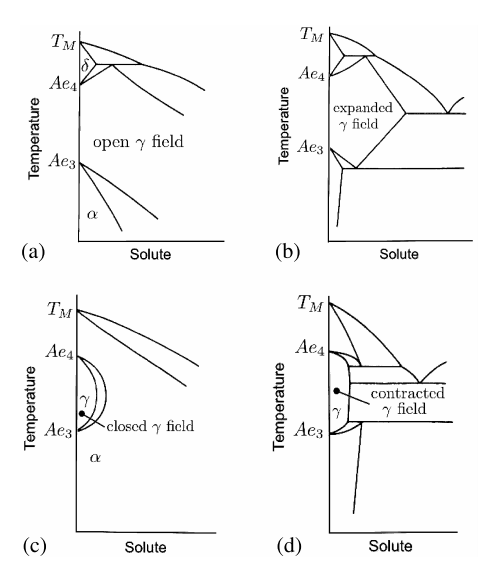
\includegraphics[width=.7\textwidth]{img/elementos-liga.png}
  \caption{Classificação dos domínios $\gamma$ sob influência dos elementos de liga: a) aberto; b) expandido; c) fechado; d) contraído. \cite{Honeycombe1982}}
  \label{fig:elem-liga}
\end{figure}

\section{Determinação das Temperaturas Críticas}

% Dada a importância de conhecer as temperaturas críticas de aços para obtenção das propriedades desejadas, foram desenvolvidas diversas formas para determiná-las.
São reportadas na literatura diversas formas de determinação de temperaturas críticas de aços, sejam de forma experimental ou computacional.

Transformações de fase do aço causam contração ou expansão do material, devido às diferentes densidades das fases que se formam ou dissolvem. A dilatometria é um método de determinação experimental de detecção de transformações de fases através da coleta de sinais de mudança nas dimensões do corpo de prova bem como sua temperatura. As temperaturas críticas de transformação podem então ser determinadas graficamente pelas inflexões nas curvas da dilatação em função da temperatura, como as mostradas na Figura \ref{fig:dilatometer}. Na Figura \ref{fig:dilatometer}, na nomenclatura utilizada pelo autor, a temperatura A1 equivale a A\textsubscript{c1p}, A1' corresponde a A\textsubscript{c1k}, e a temperatura A3 é a temperatura Ac\textsubscript{3} ou Acm. Apesar de preciso, o equipamento tem custo elevado e necessita de pessoas capacitadas para operá-lo.

\begin{figure}[ht!]
  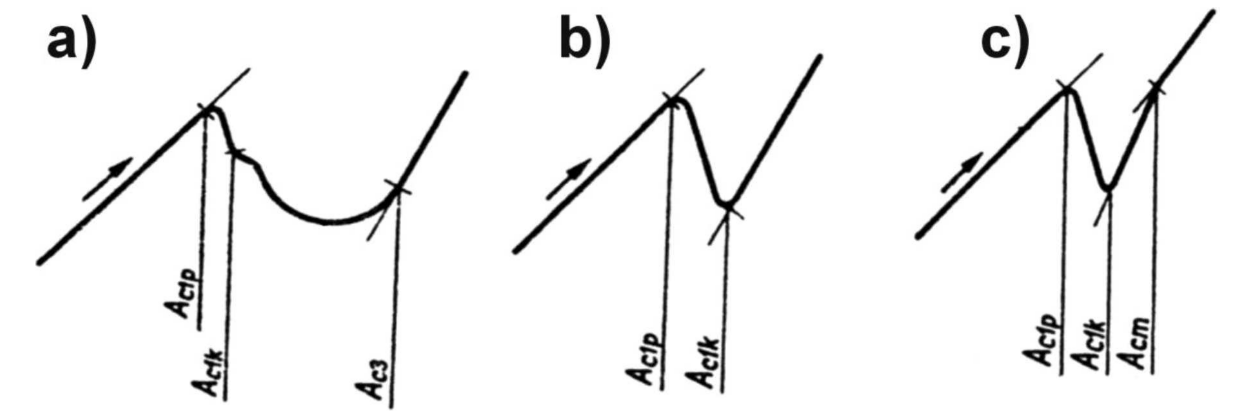
\includegraphics[width=.9\textwidth]{img/dilatometer.png}
  \caption{Determinação gráfica das temperaturas críticas em aço (a) hipoeutetóide, (b) eutetóide e (c) hipoeutetóide, a partir de dados do dilatômetro \cite{Pawlowski2012}}
  \label{fig:dilatometer}
\end{figure}

Outro método de determinar as temperaturas críticas de transformação é através de softwares de termodinâmica computacional, como o Thermo-Calc\textregistered{}, que calculam as variáveis de estado (e.g., fração de fases, composição das fases) baseados nos princípios termodinâmicos (minimização da energia livre de Gibbs). Estes softwares acessam bases de dados termodinâmicos que fornecem informações dos parâmetros de interação dos elementos químicos para determinadas fases, que então são utilizados para o cálculo da energia livre de Gibbs. A precisão dos cálculos computacionais é precisa e tem sido constantemente avaliada na literatura. Entretanto, tanto software quanto o acesso aos bancos de dados é normalmente pago, e requer-se certo aprendizado para sua manipulação.

Uma terceira maneira é a utilização de equações empíricas que se baseiam na concentração em massa dos elementos presentes no aço. A elaboração dessas equações envolve um método de regressão múltipla. \citaremsentenca{Gorni2012} compilou diversas fórmulas para o cálculo das temperaturas de transformação para austenita A1 e A3. Abaixos são mostradas duas equações para o cálculo das temperaturas A1 e A3, conforme propostas por \citaremsentenca{ANDREWS1965}:

\begin{align}
  A1 &= 723 - 16.9 Ni + 29.1 Si + 6.38 W - 10.7 Mn + 16.9 Cr + 290 As \label{eq:andrewsA1}\\
  A3 &= 910 - 203 \sqrt{C}  + 44.7 Si - 15.2 Ni + 31.5 Mo + 104 V + 13.1 W - 30.0 Mn \nonumber \\
     & + 11.0 Cr + 20.0 Cu - 700 P - 400 Al - 120 As - 400 Ti \label{eq:andrewsA3}
\end{align}

\textit{(A melhorar: detalhar melhor os métodos; inserir outras equações empíricas)}

\section{Aprendizado de m\'aquina e a determinação de Temperaturas Cr\'iticas}

Dada a complexidade e o custo de desenvolvimento de um novo material, estudos recentes têm se voltado para a tecnologia como primeira forma de avaliar hipóteses \cite{Belisle2015}. Uma vez que muitas variáveis estão envolvidas na determinação de uma propriedade, tornaram-se populares algoritmos capazes de aprender com alguma experiência vinda de um conjunto de tarefas, cujo desempenho melhora quanto maior sua experiência, também chamados de \textit{machine learning}, ou aprendizado de máquina.

Esses algoritmos podem ser classificados entre supervisionados e não supervisionados. Ele é dito supervisionado quando recebe um banco de dados com as respostas certas e a partir delas prevê um valor para dada situação (regressão) ou faz uma classificação binária. Já o algoritmo não supervisionado não sabe quais são as respostas certas; ele é alimentado com dados para que se encontre um padrão (clusterização) \footnote{Informações extraídas das vídeo aulas do curso de Machine Learning ministrado por Andrew Ng, disponível em <https://pt.coursera.org/learn/machine-learning>}.

No campo da engenharia de materiais, os algoritmos mais utilizados são os supervisionados, uma vez que pode-se reunir dados teóricos ou experimentais e a partir deles fazer a predição de propriedades. Diversas funções podem ser utilizadas para esse fim, cada uma com certa eficiência, e segundo o teorema ``No Free Lunch'' de Wolpert e Macready \enfase{apud} \citaremsentenca{Belisle2015}, não existe um algoritmo perfeito.

Dentre os métodos supervisionados, destacam-se os algoritmos que foram explorados nesse trabalho.

\subsection{Modelos de regress\~ao}

% REGRESSÃO E INTERPOLAÇÃO SÃO COISAS DISTINTAS
% O primeiro e mais simples é a interpolação polinomial. Este pode se comportar de forma linear, como descrito na equação \ref{eq:interpolacao_linear}, ou quadrática, como na equação \ref{eq:interpolacao_quadratica}.
% Este pode se comportar de forma linear, como descrito na equação \ref{eq:interpolacao_linear}, ou quadrática, como na equação \ref{eq:interpolacao_quadratica}.

% \begin{align}
%   f(x) &= b x + c \label{eq:interpolacao_linear} \\
%   f(x) &= \frac{1}{2} a x^T + b x + c \label{eq:interpolacao_quadratica}
% \end{align}

% Ambos são métodos muito utilizados devido ao baixo custo computacional. Entretanto, têm a necessidade de estabelecer alguma relação (linear ou quadrática) entre os termos estudados, utilizando termos fixos \cite{Bhadeshia1999}.

% USE O CAPÍTULO 10 DO MONTGOMERY COMO REFERÊNCIA BASE
Uma das formas mais simples de aprendizado de máquina são modelos de regressão. Uma análise de regressão procura descrever as relações entre uma variável dependente (também chamada de variável de resposta) e variáveis independentes.

Em particular, modelos de regressão linear são aqueles em que a relação entre as variáveis dependente e independentes pode ser descrita por uma relação linear do tipo:

\begin{align}
  y &= \beta_0 + \beta_1 x_1 + \beta_2 x_2 + \dots + \beta_k x_k + \epsilon \nonumber \\
    &= \beta_0 + \sum_{i=1}^k \beta_i x_i + \epsilon
  \label{eq:regressao_linear}
\end{align}
%
em que $y$ representa a variável dependente e $x_j$ e $\beta_j$ correspondem às variáveis dependentes e aos coeficientes de regressão.

O modelo de regressão também pode ser descrito por uma equação polinomial. A equação \ref{eq:regressao_polinomial_2a_ordem} abaixo representa um modelo de regressão em que a relação entre as variáveis é descrita por um polinômio de segunda ordem. Esse tipo de modelo de regressão é também chamado de modelo de superfície de reposta de segunda ordem.

\begin{equation}
  y = \beta_0 + \sum_{i=1}^k \beta_i x_i + \sum_{i=1}^{k} \sum_{j=i}^k \beta_{ij} x_i x_j + \epsilon
  \label{eq:regressao_polinomial_2a_ordem}
\end{equation}

Note-se que o modelo descrito pela equação \ref{eq:regressao_polinomial_2a_ordem} também se trata de um modelo de regressão linear, uma vez que os termos de segunda ordem podem ser redefinidos como novas variáveis independentes de primeira ordem. De forma a ilustrar melhor esta situação, tome-se como exemplo o seguinte modelo de segunda ordem com duas variáveis $x_1$ e $x_2$:

\begin{equation}
  y = \beta_0 + \beta_1 x_1 + \beta_2 x_2 + \beta_{11} {x_1}^2 + \beta_{22} {x_2}^2 + \beta_{12} x_1 x_2 + \epsilon
  \label{eq:regressao_polinomial_2a_ordem_2_var}
\end{equation}

Definindo $x_3 = {x_1}^2$, $x_4 = {x_2}^2$, $x_5 = x_1 x_2$, $\beta_3 = {\beta_1}^2$, $\beta_4 = {\beta_2}^2$ e $\beta_5 = \beta_1 \beta_2$, então a equação \ref{eq:regressao_polinomial_2a_ordem_2_var} se torna:

\begin{equation}
  y = \beta_0 + \beta_1 x_1 + \beta_2 x_2 + \beta_3 x_3 + \beta_4 x_4 + \beta_5 x_5 + \epsilon 
\end{equation}
%
que possui a mesma forma que a equação \ref{eq:regressao_linear} do modelo de regressão linear.

\textit{(Falar um pouco sobre método dos mínimos quadrados)}

% The method of least squares is typically used to estimate the regression coefficients in a mul-
% tiple linear regression model. Suppose that n 
%  k observations on the response variable are
% available, say y 1 , y 2 , . . . , y n . Along with each observed response y i , we will have an observa-
% tion on each regressor variable and let x ij denote the ith observation or level of variable x j .


\textit{(A melhorar: detalhar variáveis dependentes e independentes, regressão multivariável, métricas, overfit)}

\subsection{Rede Neural Artificial}
Um segundo método é a rede neural. Inspirada no cérebro humano, baseia-se em associações para fazer previsões, sendo muito utilizada para reconhecimento de padrões. É indicada para funções não lineares e pode identificar relações complexas entre variáveis independentes. A desvantagem é o maior tempo computacional necessário \cite{Belisle2015}.

A rede neural artificial é um conjunto de neurônios de software organizados em camadas, conectados de forma que possibilita a comunicação entre eles. Como mostra a Figura \ref{fig:rede-neural-arquitetura}, ela tem uma camada de entrada, uma ou mais camadas intermediárias e outra de saída.

\begin{figure}[ht!]
  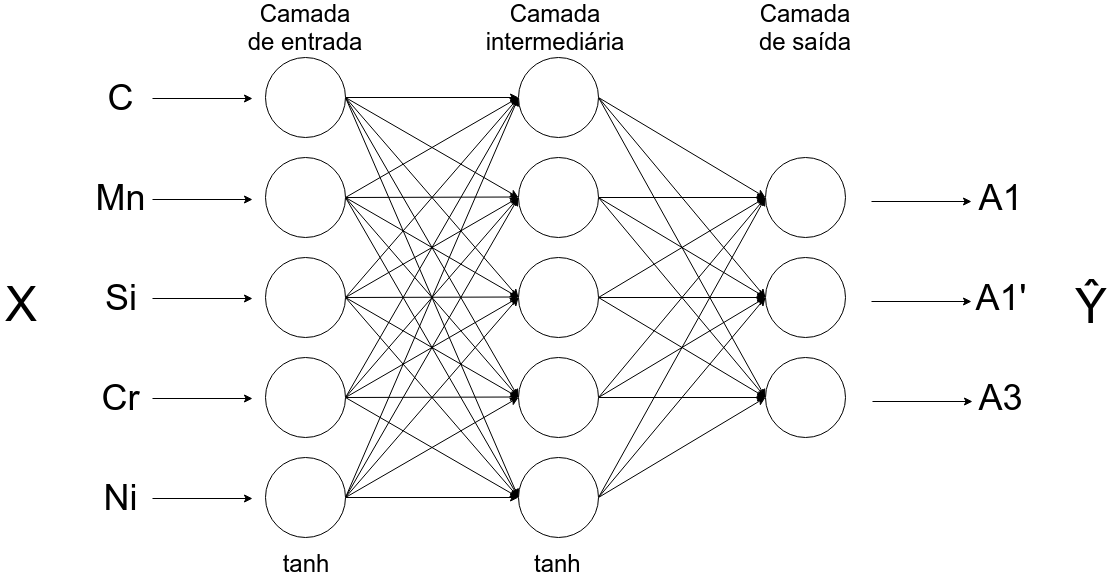
\includegraphics[width=.9\textwidth]{img/neural-network.png}
  \caption{Arquitetura da rede neural}
  \label{fig:rede-neural-arquitetura}
\end{figure}

Para o exemplo da Figura \ref{fig:rede-neural-arquitetura}, a primeira camada recebe uma entrada X de cinco dados n vezes, sendo n o tamanho do banco de dados utilizado no treinamento. Os neurônios da camada intermediária recebem o vetor X com as 5 entradas para calcular o valor predito Ŷ. Para cada neurônio existem os vetores de peso e os viéses (ou \textit{bias}), que a princípio são randômicos. O vetor X é multiplicado pelo vetor de peso e depois adicionado ao viés, como mostra a Equação \ref{eq:single-neuron}. Como os valores dos pesos e viéses são aleatórios, o valor da saída inicialmente é bem diferente do esperado. A cada iteração, os pesos são alterados até atingir um resultado satisfatório, etapa chamada de treinamento da rede neural \cite{Bhadeshia1999}.

\begin{align}
  z &= {w}_1 {x}_1 + {w}_2 {x}_2 + {w}_3 {x}_3 + ... + {w}_n {x}_n \label{eq:single-neuron}
\end{align}

Como mostra a Figura \ref{fig:single-neuron}, o resultado desse cálculo passa por uma função de ativação para que se defina a próxima conexão \cite{Skalski2017}.

\begin{figure}[ht!]
  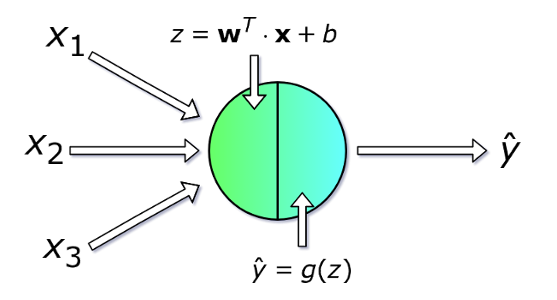
\includegraphics[width=.7\textwidth]{img/single-neuron.png}
  \caption{Operações em um único neurônio \cite{Skalski2017}}
  \label{fig:single-neuron}
\end{figure}

\citaremsentenca{Gavard1996} elaborou uma rede neural para prever A1 e A3 a partir de dados experimentais de composição química, temperatura e wtaxa de aquecimento. O modelo foi capaz de estimar temperaturas críticas com precisão de $\pm 40$K ou $95\%$ de confiança.

\textit{(A melhorar: detalhar função de ativação; falar sobre taxa de aprendizado, retropropagação, função perda, métricas de avaliação)}

\subsection{Preparação dos Dados}
\textit{(Ainda será escrito. Falar sobre separação de dados entre treino e teste e como auxilia no overfit, normalização)}

\chapter{Metodologia}

\section{O Banco de Dados}

\label{sec:banco_dados}

\subsection{Escolha das vari\'aveis}

A primeira etapa para elaboração de um algoritmo de aprendizado de máquina é a construção do banco de dados utilizado em seu treinamento. Para este trabalho, utilizou-se dados extraídos do software Thermo-Calc\textregistered{}, devido à sua acessibilidade.

Inicialmente, discutiu-se os elementos de liga e suas respectivas faixas de composição química nos aços estudados. Foram considerados apenas os mais comuns aços de engenharia, cujas composições foram consultados em um handbook SAE \cite{SAE1983}. Não foram consideradas as composições relativas aos aços inoxidáveis. A Tabela \ref{tab:faixas_composicao} mostra as faixas de composições escolhidas para criação do banco de dados de temperaturas críticas.

\begin{table}
  \caption{Faixas de composição química dos elementos de liga}

  \begin{tabular}{c c c}
  \hline
  \textbf{Elemento de liga} & \textbf{\% mínima} & \textbf{\% máxima} \\
  \hline
  Carbono & 0 & 1,5 \\
  Manganês & \SI{1e-6}{} & 3,0 \\
  Silício & \SI{1e-6}{} & 3,0 \\
  Cromo & \SI{1e-6}{} & 3,0 \\
  Níquel & \SI{1e-6}{} & 3,0 \\
  \hline
  \end{tabular}

  \label{tab:faixas_composicao}
\end{table}

Também discutiu-se a faixa de temperatura a ser estudada. Para isso, analisou-se os diagramas binários para cada elemento de liga, que podem ser encontrados no Anexo \ref{an:diag_bin}, e observou-se suas temperaturas críticas. Considerando a temperatura em que pode ser observada austenita, utilizou-se o intervalo de 673 a 1473K.

Definidas as faixas de composição química e temperatura, foram definidos os níveis para cada elemento, ou seja, quantas variações (ou passos) cada elemento tem. O valor do passo é dado pela equação a seguir:

\begin{equation}
  passo = \frac{\Delta c}{n - 1}
\end{equation}

Assim, os níveis e passos utilizados para cada elemento são dados na Tabela \ref{tab:niveis_e_passos}.

\begin{table}
  \caption{Níveis e passos para cada elemento de liga}

  \begin{tabular}{c c c}
  \hline
  \textbf{Elemento de liga} & \textbf{Níveis} & \textbf{Valor do passo} \\
  \hline
  Carbono & 11 & 0,15 \\
  Manganês & 5 & 0,75 \\
  Silício & 5 & 0,75 \\
  Cromo & 5 & 0,75 \\
  Níquel & 5 & 0,75 \\
  \hline
  \end{tabular}

  \label{tab:niveis_e_passos}
\end{table}

Já para a temperatura, estabeleceu-se um passo de 10K. A partir da combinação desses valores de composição, um script faz a chamada do Thermo-Calc\textregistered{}. Dessa forma, para dada composição química, são retornadas as porcentagens de cada fase (ferrita, austenita e cementita) para cada temperatura dentro da faixa estabelecida. O resultado da chamada do Thermo-Calc\textregistered{} é salvo em um arquivo de texto de extensão ``.DAT''. No total, foram gerados 6875 arquivos.

\subsection{Extra\c{c}\~ao de temperaturas cr\'iticas}

Para cada arquivo gerado pela chamada do Thermo-Calc\textregistered{}, as temperaturas críticas foram calculadas por meio de outro script. Este faz a leitura do arquivo .DAT, que contém as porcentagens de cada fase para cada temperatura entre 673 e 1473K, variando em 10K.

Para determinar a A1, identifica-se a maior temperatura em que a porcentagem de austenita é zero, enquanto que para a temperatura A3, identifica-se a menor temperatura em que a porcentagem de austenita é 100\%. Também identificou-se a temperatura crítica intermediária, A1', e se o aço da respectiva simulação é hipo ou hipereutetóide. Para isso, comparou-se a temperatura em que a porcentagem de ferrita é zero ($T_{ferr}$) com a que a porcentagem de cementita é zero ($T_{cem}$). Caso $T_{ferr}$ seja maior que $T_{cem}$, A1' é igual a $T_{cem}$ e o aço é hipoeutetóide; caso contrário, A1' é igual a $T_{ferr}$ e o aço é hipereutetóide. Uma terceira situação é a aquela em que não há cementita para a composição dada e assim não há campo trifásico e A1' seria igual a A1.

Os dados do nome do arquivo, o número da macro que fez sua chamada, composição química, temperaturas críticas e classificação em hipo ou hiper eutetóide foram salvos em um arquivo CSV.

\subsection{Avaliação do banco de dados}

Foram realizados testes para averiguar a qualidade dos dados extraídos do Thermo-Calc\textregistered{}.

Para avaliar a coerência, foi elaborado um script que plota simultaneamente o gráfico da porcentagem de austenita em função da temperatura, comparando dados da tabela de resultado com dados de uma única chamada do Thermo-Calc\textregistered{}. Dessa forma, foi possível testar resultados pontuais considerados inconsistentes.

Outro teste realizado foi a verificação da existência das fases ferrita, austenita e cementita, para averiguar quais composições poderiam ser problemáticas para determinar as temperaturas críticas.

Uma importante verificação da base de dados como um todo foi a comparação com os resultados das equações empíricas de Andrews. Para cada composição química do banco de dados, calculou-se as temperaturas críticas A1 e A3 pelas equações empíricas. A partir disso, gerou-se um gráfico de temperatura crítica calculada versus temperatura crítica gerada pelo Thermo-Calc\textregistered{}.

A fim de avaliar o efeito de cada elemento na temperatura crítica A3, foram traçadas isopletas com a composição de carbono como variável livre e diferentes composições de cada elemento.

\section{Regressão Linear}
\label{sec:metodo_RL}

Analisou-se a predição das temperaturas A1, A1' e A3 atráves de algoritmos de regressão linear multivariável.

Primeiramente, o banco de dados gerado conforme a secção \ref{sec:banco_dados} foi manipulado, transformando as composições para porcentagem em peso e as temperaturas para graus Celsius, além de remover os dados cujas temperaturas críticas não existissem. A fim de avaliar o efeito dos termos ao quadrado e da interdependência entre elementos químicos no valor das temperaturas críticas, foram criadas novas colunas, totalizando os seguintes parâmetros: C, $C^{2}$, CMn, CSi, CCr, CNi, Mn, $Mn^{2}$, MnSi, MnCr, MnNi, Si, $Si^{2}$, SiCr, SiNi, Cr, $Cr^{2}$, CrNi, Ni, $Ni^{2}$.

Em seguida, o banco de dados foi separado entre dados de treino e dados de teste para o algoritmo. Utilizou-se a proporção 80\% treino e 20\% teste, selecionando dados com um algoritmo pseudoaleatório, ou seja, para uma mesma semente são selecionados os mesmos dados.

Na sequência, os dados de treino foram utilizados para gerar modelos de regressão linear multivariável, utilizando o \textit{Scikit-learn}. Essa biblioteca do \textit{Python} contém funções eficientes de aprendizado de máquina, incluindo o módulo \textit{linear\_model}, no qual se espera que o valor alvo seja uma combinação linear dos dados de entrada.

Para cada temperatura crítica, foi gerado um modelo para composições hipoeutetóides, um para hipereutetóides e um para todas as composições, totalizando nove modelos. Para cada modelo obteve-se os coeficientes de regressão de cada variável independente e calculou-se o coeficiente de determinação ($R^{2}$) da predição do modelo.

Para cada modelo, foram plotados gráficos de valores preditos versus valores esperados para o conjunto de dados de teste, além de isopletas de A3 com os dados de treino e de teste, para posterior comparação com as isopletas da rede neural. Para a isopleta do carbono, utilizou-se tanto o modelo hipoeutetóide quanto hipereutetóide para prever o valor de A3 para os demais elementos no nível zero. Já para as demais isopletas, utilizou-se apenas o modelo hipoeutetóide, pois para nível zero de carbono não há aços hipereutetóides.

Visto que os valores de $R^{2}$ foram muito satisfatórios, realizou-se um novo teste, a fim de verificar a possibilidade de \textit{overfit}. Para isso, gerou-se um novo banco de dados de teste, de tamanho equivalente a 20\% ao do banco original, utilizando o algoritmo \textit{rand} do \textit{Numpy}, que retorna números aleatórios distribuídos uniformemente de 0 a 1. Em seguida esses números foram multiplicados pelas composições máximas do elemento químico correspondente, a fim de se obter ligas dentro das faixas de composição estudadas. Por fim, foram rodados os scripts para determinar a temperatura dada pelo Thermo-Calc\textregistered{}, descritos na secção \ref{sec:banco_dados}. Novos cálculos de $R^{2}$ foram feitos e comparados com os originais.

\section{Rede Neural}
Dado que a temperatura A3 é a mais complexa de se determinar, devido à inversão da curva no ponto eutetóide, para essa temperatura crítica foi elaborada uma rede neural, de arquitetura semelhante à mostrada na Figura \ref{fig:rede-neural-arquitetura}.

Para isso, houve o mesmo tratamento de dados descrito na secção \ref{sec:metodo_RL}, transformando as composições para porcentagem em peso, as temperaturas para graus Celsius, e removendo os dados cujas temperaturas críticas não existissem. Também foi feita a mesma separação entre dados de treino e teste, utilizando a mesma proporção de 80/20\%, respectivamente.

Além desses procedimentos, a rede neural exige que os dados sejam normalizados para que haja melhor convergência, uma vez que a função de ativação escolhida para o modelo foi a de tangente hiperbólica. Foi utilizado o \textit{MinMax Scaler}, função do módulo \textit{Scikit-learn} do \textit{Python}, que reduz o intervalo dos dados para que estejam entre 0 e 1.

Para construção da rede neural, foi utilizado o Keras, uma API de alto nível escrita em \textit{Python} e cujo
\textit{backend} pode ser rodado em \textit{TensorFlow}, \textit{CNTK} ou \textit{Theano}. Para esse caso, foi utilizado o \textit{TensorFlow}. Essa biblioteca tem como maior vantagem a agilidade para criar modelos complexos, facilitando a elaboração de testes \cite{Skalski2017}.

Como valor de saída foi estabelecido A3, enquanto as porcentagens em peso de C, Mn, Si, Cr, Ni foram definidas como valores de entrada. Foram variados o número de neurônios na camada intermediária, de 1 a 12, bem como a taxa de aprendizado (ou \textit{learning rate}) de 0.1, 0.01 e 0.001. Foram plotados gráficos de Erro quadrático médio versus número de neurônios na camada intermediária, com o intuito de estipular um ponto ótimo desses parâmetros, como realizado no trabalho de \citaremsentenca{Capdevila2004}. Para um mesmo número de neurônios, foram testados 5 modelos, uma vez que os pesos e vieses iniciais são aleatórios e podem influenciar no resultado final.

Definida a taxa de aprendizado que apresentava melhor estabilidade do erro quadrático médio, avaliou-se o efeito do número de neurônios na camada interna na função perda e nos valores preditos. Foram plotados gráficos de função perda versus número de iterações, bem como de valores preditos versus valores esperados, para número de neurônios na camada intermediária de 1 a 12.

Estabelecendo o ponto ótimo de número de neurônios, foram plotadas isopletas comparando os dados de treino com de teste, foram calculados o coeficiente de determinação ($R^{2}$) e o erro quadrático médio (MSE) da predição do modelo.

\section{Comparação dos modelos}

Para se comparar a assertividade dos modelos, foram comparados os coeficientes de determinação de regressão linear e rede neural para predição da temperatura A3.

Também foram plotados gráficos de valores preditos pela regressão linear e pela rede neural versus valores calculados pela equação empírica, uma vez que os dados normalizados não podem ser usados para essas equações e a comparação das métricas não teria sentido. Para isso, as predições da rede neural foram desnormalizadas utilizando o método \textit{inverse\_transform} do \textit{Scikit-learn}.

 %ARRUMAR: falar quais equações usou

\chapter{Resultados e discussão}

\section{O Banco de Dados}

O resultado da variação de composição química para aços carbono gerou um total de 6875 combinações e, para cada, fez-se a chamada do Thermo-Calc\textregistered{} que retorna a porcentagem de cada fase para temperaturas de 673 a 1473K, variando de 10K. Para cada composição, os dados são salvos em um arquivo .DAT.

Inicialmente, sete macros faziam a chamada do Thermo-Calc\textregistered{} com 1000 composições cada. Isso trouxe resultados muito inconsistentes, como valores em branco ou ou incoerentes com a literatura, e podem estar relacionados à sobrecarga de memória do computador. Notou-se que, quanto menos chamadas cada macro fazia, menor o número de erros nos resultados e, assim, chegou-se ao número de 69 macros com 100 chamadas cada.

Em seguida, para cada arquivo, extraiu-se as temperaturas críticas A1, A1' e A3. A Figura \ref{fig:Tcrit_exemplos} ilustra a lógica dessa extração. A temperatura A1' é representada pela mudança de inclinação na curva da porcentagem de austenita. Para aços hipoeutetóides, essa temperatura corresponde ao ponto em que a porcentagem de cementita é zero, como mostra a Figura \ref{fig:Tcrit_exemplos}a. Já para hipereutetóides, ao ponto em que a porcentagem de ferrita é zero, como na Figura \ref{fig:Tcrit_exemplos}b. Enquanto isso, para aços em que a porcentagem de cementita é sempre zero, considera-se que a temperatura A1' é igual à A1 (vide Figura \ref{fig:Tcrit_exemplos}c).

\begin{figure}
  \subfloat[]{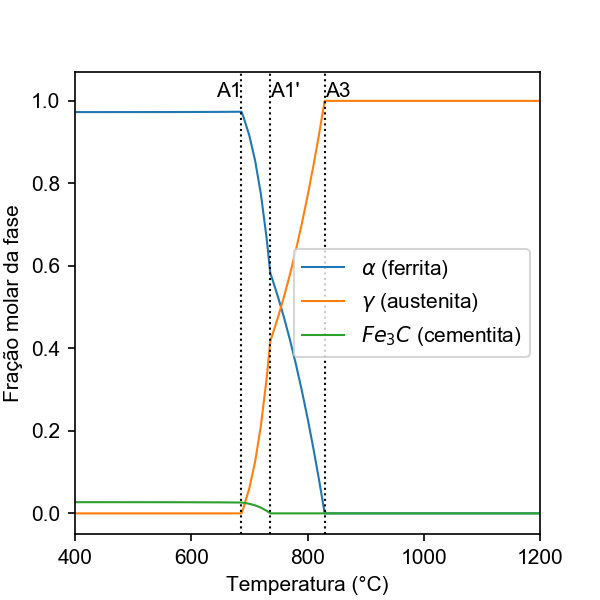
\includegraphics[width=.5\textwidth]{img/alloy_hipo.png}}\hfill
  \subfloat[]{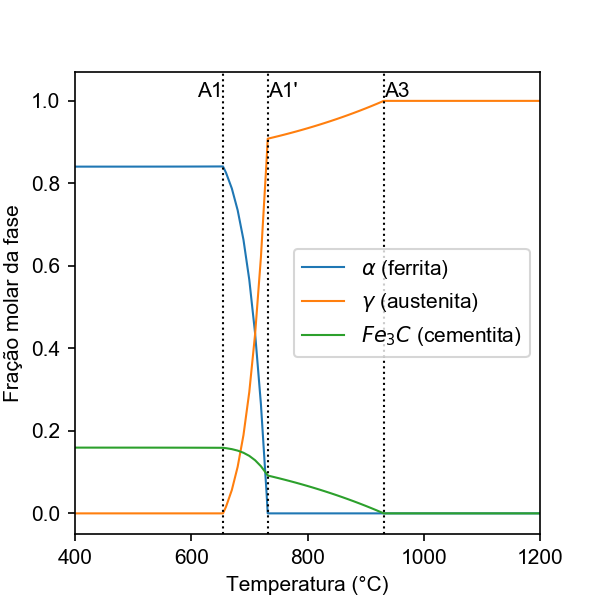
\includegraphics[width=.5\textwidth]{img/alloy_hiper.png}}\\
  \subfloat[]{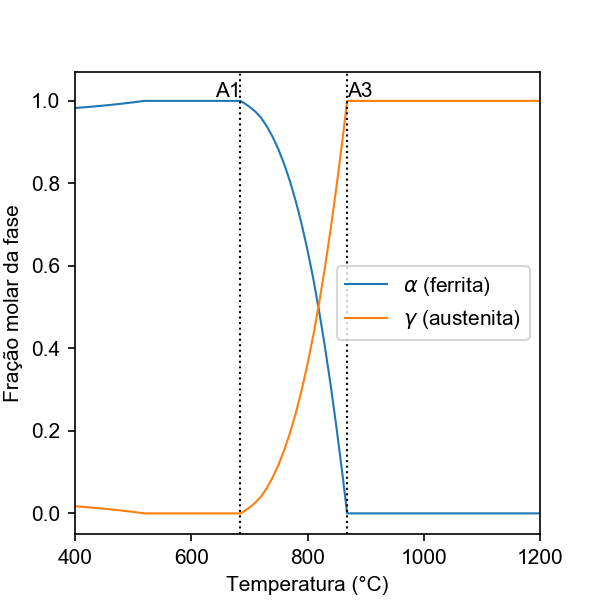
\includegraphics[width=.5\textwidth]{img/alloy_nocem.png}}
  \caption{Exemplos de extração de temperaturas críticas para a) liga hipoeutetóide, b) liga hipereutetóide e c) liga hipoeutetóide sem cementita}
  \label{fig:Tcrit_exemplos}
\end{figure}


É importante destacar que nem sempre um aço terá as três temperaturas críticas. Elementos muito alfagênicos podem não ter A3, como no caso de um $\gamma$ loop, e gamagênicos podem não ter A1, por terem austenita estável à temperatura ambiente.

Mesmo considerando que algumas temperaturas críticas podem não existir para certas composições, ainda não se sabe as causas dos erros que ocorreram nessa extração. Por exemplo, algumas composições com baixo carbono ficaram com valores em branco, enquanto outras tiveram valores de temperatura crítica muito acima do esperado, embora os gráficos plotados para sua respectiva composição estivessem dentro do esperado. Assim, foi feito um script que faz essa correção, fazendo apenas uma chamada do Thermo-Calc\textregistered{} por vez.

% \subsection{Comparação com equações empíricas}

Foi realizada uma comparação dos valores de temperatura crítica com a equação empírica de Andrews, plotando o gráfico da Figura \ref{fig:tcrit_andrews}. A linha em azul representa os valores esperados ($T_{empirical} = T_{database}$).

\begin{figure}
  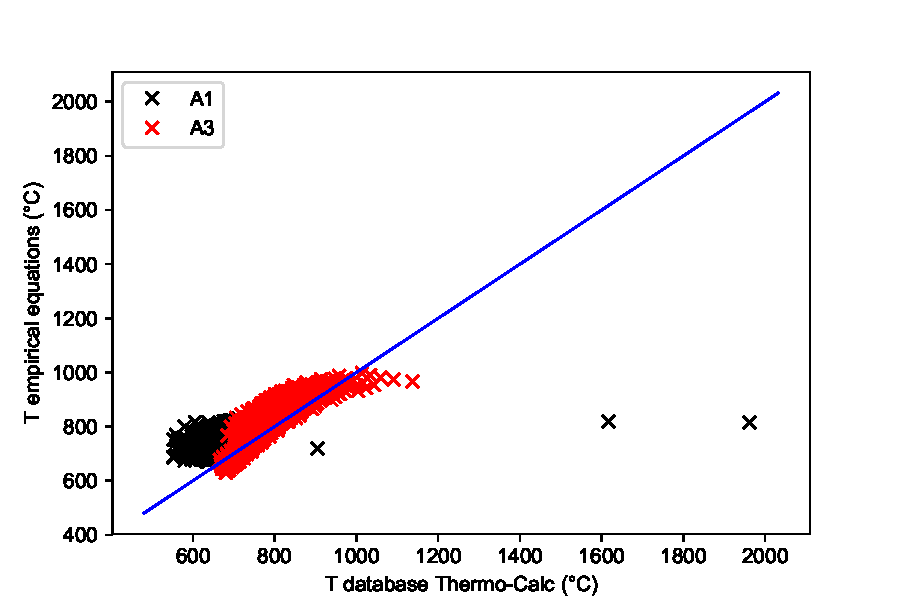
\includegraphics[width=1.1\textwidth]{img/andrews.pdf}
  \caption{Gráfico de temperatura crítica calculada pela equação empírica de Andrews e temperatura crítica do banco de dados}
  \label{fig:tcrit_andrews}
\end{figure}

Nota-se que, para as temperaturas A3, existe uma correlação maior com os valores calculados pela equação empírica, enquanto para A1 existe uma divergência maior. Isso pode estar relacionado com o fato de a equação de Andrews não ter membros interdependentes entre os elementos químicos, o que na prática não se aplica.

Para averiguar essa interdependência, plotou-se as isopletas de temperatura para cada elemento, variando a composição de carbono. Para cada elemento de liga, plotou-se cinco curvas, correspondentes aos cinco níveis de composição escolhidos.

Para o manganês e níquel, nota-se que a baixas concentrações de carbono a concentração do elemento de liga tem muita interferência no valor das temperaturas de transformação. A partir de 0,8\% C, as temperaturas são mais próximas para todos os níveis. Uma possível explicação é que os três elementos são gamagênicos.

Já para elementos alfagênicos, como o cromo, a relação se inverte. Para baixas concentrações de carbono, os valores de temperatura ficam próximos, e a partir de 0,4\% de carbono a concentração do cromo já contribui para sua divergência.

Um caso intermediário é o do silício, que apesar de alfagênico, tem influência na temperatura tanto a baixas quanto a mais altas concentrações de carbono, embora a influência a baixas concentrações seja maior.

\textit{(A melhorar: inserir isopletas do banco de dados)}

\section{Regressão Linear}

Após o tratamento dos dados, pontos cuja temperatura crítica correspondente não existisse foram eliminados e os
dados foram separados entre hipo e hipereutetóide. A Tabela \ref{tab:conj_dados} mostra o tamanho do banco de dados para cada condição.

\begin{table}
  \caption{Tamanho dos conjuntos de dados usados para regressão linear}

  \begin{tabular}{llll}
  \hline
                 & A1   & A1'  & A3   \\
  \hline
  Hipoeutetóide  & 1151 & 1643 & 2303 \\
  Hipereutetóide & 3308 & 4339 & 4542 \\
  Total          & 4459 & 5982 & 6845 \\
  \hline
  \end{tabular}

  \label{tab:conj_dados}
\end{table}

Os valores de $R^{2}$ para os nove modelos são mostrados na Tabela \ref{tab:r2_reg_lin} a seguir.

\begin{table}
  \caption{Valores de $R^{2}$ para regressão linear}

  \begin{tabular}{llll}
  \hline
  & A1     & A1'    & A3     \\
  \hline
  Hipoeutetóide  & 0.8663 & 0.9743 & 0.9607 \\
  Hipereutetóide & 0.9817 & 0.9934 & 0.9971 \\
  Todos os dados & 0.9425 & 0.9748 & 0.8774 \\
  \hline
  \end{tabular}

  \label{tab:r2_reg_lin}
\end{table}

Nota-se que o conjunto de dados para determinar a temperatura A1 é o menor. Isso ocorre pois três dos cinco elementos estudados são gamagênicos, reduzindo a probabilidade de existir A1. A quantidade reduzida de dados teve efeito no valor de $R^{2}$, o menos satisfatório dos modelos, principalmente para os pontos hipoeutetóides.

Os valores de $R^{2}$ obtidos foram satisfatórios porém muito altos, por isso houve o cuidado em se verificar a possibilidade de \textit{overfit}, como será mostrado a seguir.

%ARRUMAR: adicionar tabelas com coeficientes das Regressões
\subsection{Regressão Linear de A1}

A Figura \ref{fig:LR_A1} a seguir mostra os gráficos de valores preditos versus esperados para a temperatura A1.

\begin{figure}[!h]
\subfloat[\label{fig:LR_A1_hipo}]{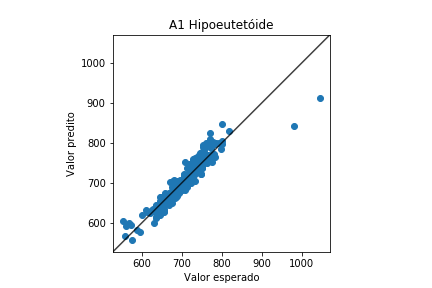
\includegraphics[width=.5\textwidth]{img/A1_hipo.png}}\hfill
\subfloat[\label{fig:LR_A1_hiper}]{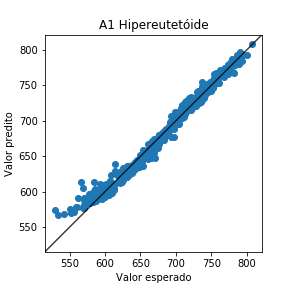
\includegraphics[width=.5\textwidth]{img/A1_hiper.png}}\\
\subfloat[\label{fig:LR_A1_total}]{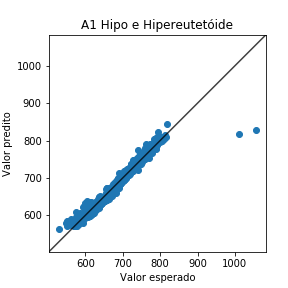
\includegraphics[width=.5\textwidth]{img/A1_total.png}}
\caption{Valores preditos vs. Valores esperados da regressão linear de A1, para (a) Hipoeutetóides, (b) Hipereutetóides, (c) Todos os valores}
\label{fig:LR_A1}
\end{figure}

Nota-se que, mesmo com a quantidade de dados reduzida, esses tiveram um bom ajuste com a reta $y = x$. Os problemas estão localizados no extremo inferior, onde a curva de A1 no diagrama binário Fe-C não se assemelha a uma reta. Essa faixa corresponde às temperaturas mais baixas dos hipoeutetóides, onde há poucos pontos devido à proximidade do campo $\alpha$, no qual A1 não existe.

\subsection{Regressão Linear de A1'}

A Figura \ref{fig:LR_A1prime} a seguir mostra os gráficos de valores preditos versus esperados para a temperatura A1'.

\begin{figure}[!h]
\subfloat[\label{fig:LR_A1prime_hipo}]{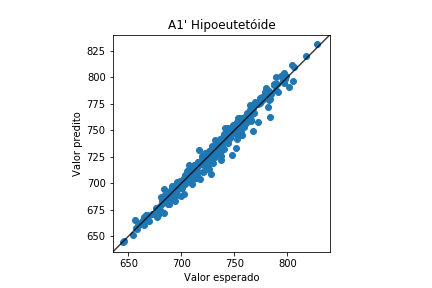
\includegraphics[width=.5\textwidth]{img/A1prime_hipo.png}}\hfill
\subfloat[\label{fig:LR_A1prime_hiper}]{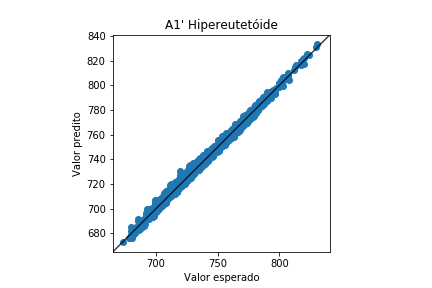
\includegraphics[width=.5\textwidth]{img/A1prime_hiper.png}}\\
\subfloat[\label{fig:LR_A1prime_total}]{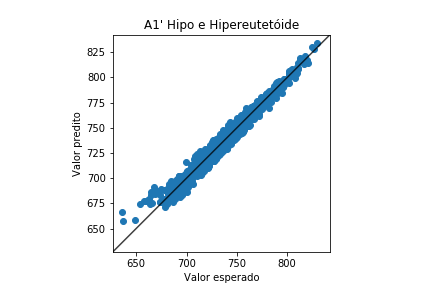
\includegraphics[width=.5\textwidth]{img/A1prime_total.png}}
\caption{Valores preditos vs. Valores esperados da regressão linear de A1', para (a) Hipoeutetóides, (b) Hipereutetóides, (c) Todos os valores}
\label{fig:LR_A1prime}
\end{figure}
% ARRUMAR: GRÁFICO NO LUGAR ERRADO

A temperatura A1', assim como A1, é mais difícil de ser determinada na proximidade do campo $\alpha$, como é possível notar nas temperaturas mais baixas dos hipoeutetóides. O maior número de dados utilizados para o treino resultou em um melhor ajuste das curvas.

\subsection{Regressão Linear de A3}

A Figura \ref{fig:LR_A3} a seguir mostra os gráficos de valores preditos versus esperados para a temperatura A3.

\begin{figure}[!h]
\subfloat[\label{fig:LR_A3_hipo}]{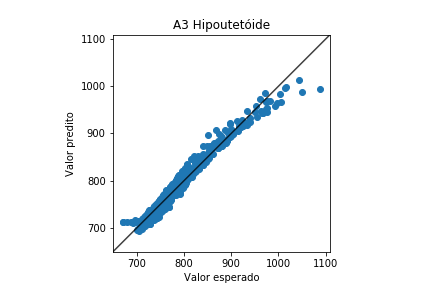
\includegraphics[width=.5\textwidth]{img/A3_hipo.png}}\hfill
\subfloat[\label{fig:LR_A3_hiper}]{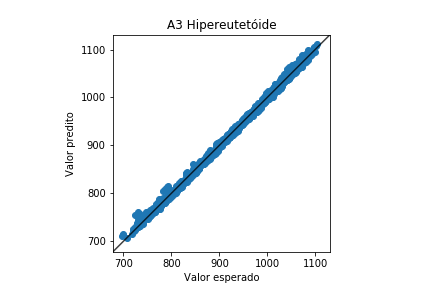
\includegraphics[width=.5\textwidth]{img/A3_hiper.png}}\\
\subfloat[\label{fig:LR_A3_total}]{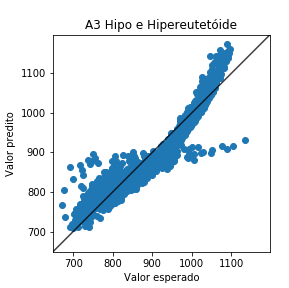
\includegraphics[width=.5\textwidth]{img/A3_total.png}}
\caption{Valores preditos vs. Valores esperados da regressão linear de A3, para (a) Hipoeutetóides, (b) Hipereutetóides, (c) Todos os valores}
\label{fig:LR_A3}
\end{figure}

Para essa temperatura crítica, os pontos que menos se ajustaram foram os hipoeutetóides. Isso possivelmente ocorre pois a curva correspondente no diagrama binário Fe-C tem uma inclinação mais variável do que a hipereutetóide. Além disso, nota-se menor quantidade de pontos a temperaturas altas, ou seja, a baixas concentrações de carbono. As predições para composições hipereutetóides tiveram melhor ajuste, não apenas pelo maior conjunto de dados mas também pela curva correspondente no diagrama binário Fe-C ter inclinação mais constante.

O modelo que utilizou todo o conjunto de dados não teve um bom ajuste, como era esperado, devido à inversão da curva no ponto eutetóide do diagrama binário Fe-C

\subsection{Comparação com banco de dados aleatórios}
Ao todo foram gerados 1375 dados de teste, que passaram novamente pela predição para se avaliar os ajustes. As Tabelas \ref{tab:r2_A1_RL_random}, \ref{tab:r2_A1prime_RL_random} e \ref{tab:r2_A3_RL_random} a seguir mostram os novos valores de $R^{2}$ recalculados para cada modelo.

\begin{table}
  \caption{Valores de $R^{2}$ para regressão linear de A1 com dados aleatórios}

  \begin{tabular}{lll}
  \hline
                 & Original & Aleatório \\
  \hline
  Hipoeutetóide  & 0.8663   & 0.7304    \\
  Hipereutetóide & 0.9817   & 0.9806    \\
  Todos os dados & 0.9425   & 0.9752    \\
  \hline
  \end{tabular}

  \label{tab:r2_A1_RL_random}
\end{table}

\begin{table}
  \caption{Valores de $R^{2}$ para regressão linear de A1' com dados aleatórios}

  \begin{tabular}{lll}
  \hline
                 & Original & Aleatório \\
  \hline
  Hipoeutetóide  & 0.9743   & 0.8137    \\
  Hipereutetóide & 0.9934   & 0.9941    \\
  Todos os dados & 0.9748   & 0.8754    \\
  \hline
  \end{tabular}

  \label{tab:r2_A1prime_RL_random}
\end{table}

\begin{table}
  \caption{Valores de $R^{2}$ para regressão linear de A3 com dados aleatórios}

  \begin{tabular}{lll}
  \hline
                 & Original & Aleatório \\
  \hline
  Hipoeutetóide  & 0.9607   & 0.9603    \\
  Hipereutetóide & 0.9971   & 0.9981    \\
  Todos os dados & 0.8774   & 0.9207    \\
  \hline
  \end{tabular}

  \label{tab:r2_A3_RL_random}
\end{table}

Os resultados obtidos dos dados aleatórios possibilitou uma comparação de métricas, uma vez que não foi encontrado na literatura o que seria um valor satisfatório de $R^{2}$ para a predição dessas temperaturas em específico. Nota-se que não houve muita variação dos valores originais para os aleatórios, entretanto, a hipótese de \textit{overfit} não pode ser completamente descartada. É possível que a alta complexidade do modelo, devido ao grande número de dados de entrada, esteja elevando as métricas.

\subsection{Isopletas das Regressões Lineares}

As predições dos modelos de A3 foram utilizadas para gerar isopletas variando-se um dos elementos e fixando os demais a nível zero. Na figura \ref{fig:LR_isopleths} a seguir, a linha azul corresponde às predições do modelo hipoeutetóide e a vermelha ao hipereutetóide, enquanto os pontos em ``x'' são os valores obtidos pelo Thermo-Calc\textregistered{}.

% ARRUMAR: gráfico na página errada
\begin{figure}[!h]
\subfloat[\label{fig:LR_isop_C}]{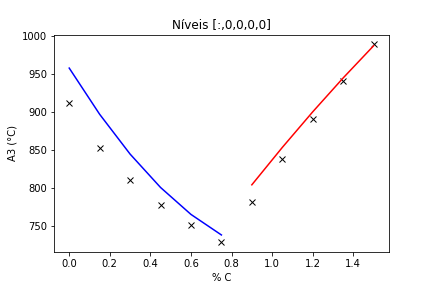
\includegraphics[width=.7\textwidth]{img/LR_C0.png}}

\subfloat[\label{fig:LR_isop_Mn}]{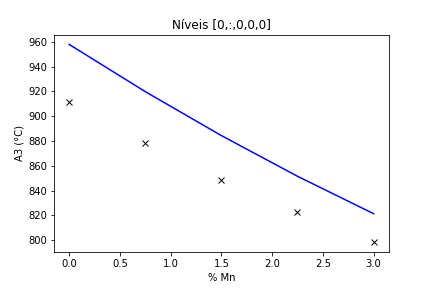
\includegraphics[width=.5\textwidth]{img/LR_Mn0.png}}
\subfloat[\label{fig:LR_isop_Si}]{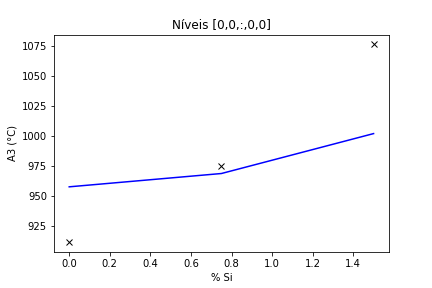
\includegraphics[width=.5\textwidth]{img/LR_Si0.png}}

\subfloat[\label{fig:LR_isop_Cr}]{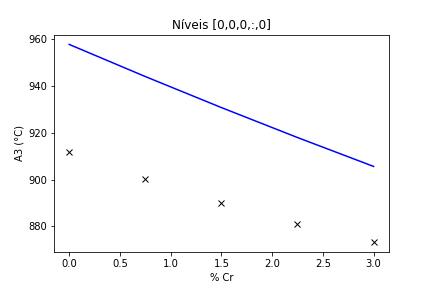
\includegraphics[width=.5\textwidth]{img/LR_Cr0.png}}
\subfloat[\label{fig:LR_isop_Ni}]{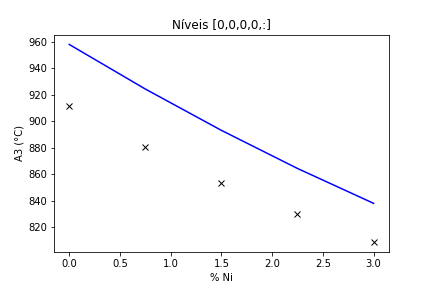
\includegraphics[width=.5\textwidth]{img/LR_Ni0.png}}
\caption{Isopletas de A3 geradas pelas predições da regressão linear para (a) Carbono; (b) Manganês; (c) Silício; (d) Cromo; (e) Níquel, a nível zero dos demais elementos}
\label{fig:LR_isopleths}
\end{figure}

Para o Carbono, a predição é próxima do esperado, principalmente para hipereutetóides. Já para hipoeutetóides, quanto menor a composição de carbono, maior a diferença entre o predito e o esperado, chegando a \SI{50}{\celsius}. Como discutido anteriormente, há uma mudança de inclinação na curva do diagrama binário Fe-C que contribui para uma má predição do modelo.

Já para o Manganês, Cromo e Níquel, as predições mantém a mesma inclinação do esperado, porém com uma diferença que chega a \SI{50}{\celsius}. O Silício, por sua vez, não teve uma boa predição, possivelmente devido ao seu domínio $\gamma$ fechado que gera um $\gamma$-\textit{loop}.
% ARRUMAR: não sei mais o que escrever aqui.

\section{Rede Neural}
Após o tratamento do banco, foram obtidos 6845 dados normalizados, que foram separados entre 5476 para treino e 1369 de teste. Os parâmetros da rede neural foram variados para se definir o melhor modelo.

\subsection{Testes para obtenção do modelo}

Avaliando-se o efeito da taxa de aprendizado e do número de neurônios da camada intermediária no erro quadrático médio, obteve-se os
gráficos da Figura \ref{fig:test_NN} abaixo.

\begin{figure}[!h]
\subfloat[\label{fig:test1}]{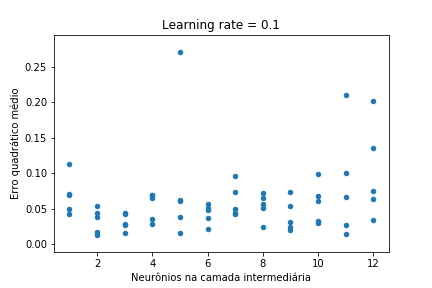
\includegraphics[width=.5\textwidth]{img/test1.png}}\hfill
\subfloat[\label{fig:test01}]{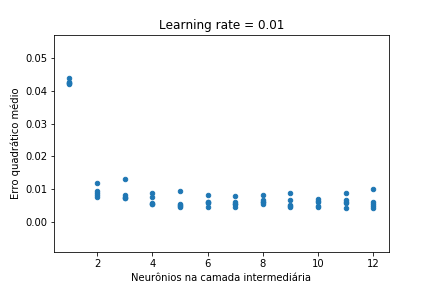
\includegraphics[width=.5\textwidth]{img/test01.png}}\\
\subfloat[\label{fig:test001}]{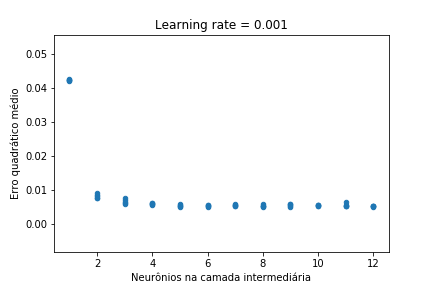
\includegraphics[width=.5\textwidth]{img/test001.png}}
\caption{Erro quadrático médio vs. Número de neurônios na camada intermediária para (a) Taxa de aprendizado = 0.1, (b)Taxa de aprendizado = 0.01, (c) Taxa de aprendizado = 0.001}
\label{fig:test_NN}
\end{figure}

Nota-se que, à medida em que a taxa de aprendizado diminui, a variação do erro quadrático médio diminui para um mesmo número de neurônios. Dessa forma, determinou-se o valor ideal para a taxa de aprendizado, 0.001.
Em seguida, foi avaliado o efeito do número de iterações e do número de neurônios na função perda. A Figura \ref{fig:loss_NN} a seguir mostra o comportamento da função perda com o número de iterações para um, seis e doze neurônios.

\begin{figure}[!h]
\subfloat[\label{fig:loss1}]{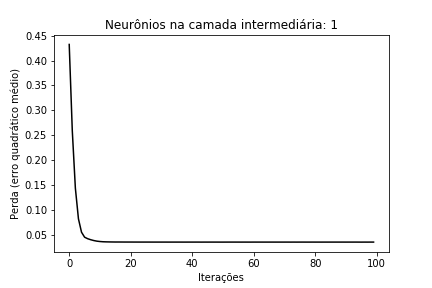
\includegraphics[width=.5\textwidth]{img/loss_1.png}}\hfill
\subfloat[\label{fig:loss6}]{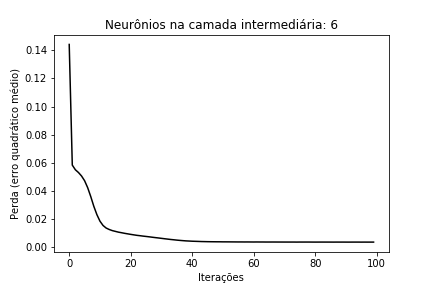
\includegraphics[width=.5\textwidth]{img/loss_6.png}}\\
\subfloat[\label{fig:loss12}]{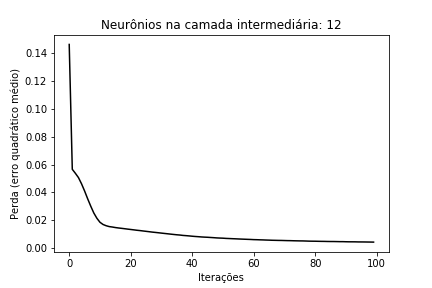
\includegraphics[width=.5\textwidth]{img/loss_12.png}}
\caption{Perda (erro quadrático médio) vs. Número de iterações para (a) 1, (b) 6, (c) 12 neurônios na camada intermediária}
\label{fig:loss_NN}
\end{figure}

Pode-se constatar que para poucos neurônios a função perda se estabiliza com menos iterações, porém a um valor maior. Aumentando-se número de neurônios, as 100 iterações se tornam cada vez mais necessárias para se obter um valor adequado de perda.

Considerando a taxa de aprendizado escolhida, nota-se que o erro quadrático médio estabiliza a partir de cinco neurônios e que 100 iterações são o suficiente para se obter uma perda adequada. Dessa forma, foi estabelecido que o ponto ótimo seria de seis neurônios e 100 iterações, considerando também o tempo computacional.

Para confirmar se esses parâmetros eram adequados, foram analisados os valores preditos versus esperados variando o número de neurônios. A Figura \ref{fig:predict_NN} a seguir mostra esse comportamento para um, seis e doze neurônios, onde os círculos preenchidos mostram os dados de treino e os triângulos, os de teste.

%ARRUMAR: FIGURA NO LUGAR ERRADO
\begin{figure}[!h]
\subfloat[\label{fig:predict1}]{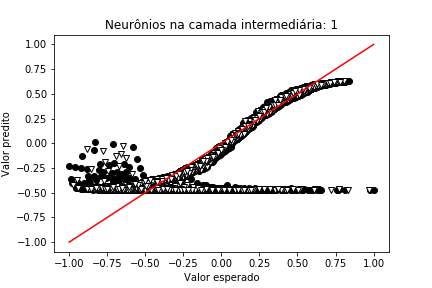
\includegraphics[width=.5\textwidth]{img/predict_1.png}}
\subfloat[\label{fig:predict6}]{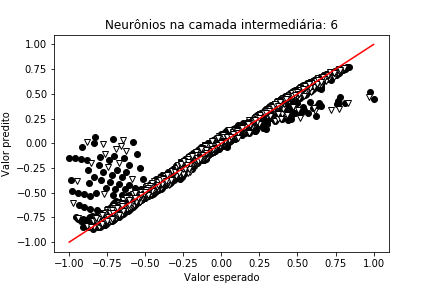
\includegraphics[width=.5\textwidth]{img/predict_6.png}}

\subfloat[\label{fig:predict12}]{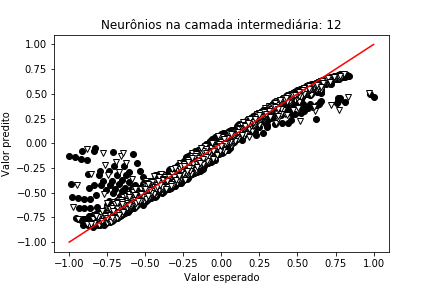
\includegraphics[width=.5\textwidth]{img/predict_12.png}}
\caption{Valores Preditos vs. Valores Esperados para (a) 1, (b) 6, (c) 12 neurônios na camada intermediária. $\bullet$ : valores de treino, $\triangledown$ : valores de teste}
\label{fig:predict_NN}
\end{figure}

Nota-se que as predições para seis e doze neurônios são próximas e, considerando o tempo computacional, a primeira opção é, de fato, o ponto ótimo.

\subsection{Isopletas da Rede Neural}

Definindo todos os parâmetros, as predições do modelo escolhido foram usadas para plotar isopletas variando um dos elementos e fixando os demais, com o intuito de se comparar os valores obtidos pelo Thermo-Calc\textregistered{} com essas predições. Como mostram as Figuras \ref{fig:C_NN_isop}, \ref{fig:Mn_NN_isop}, \ref{fig:Si_NN_isop}, \ref{fig:Cr_NN_isop} e \ref{fig:Ni_NN_isop} os elementos variáveis foram plotados nas composições de nível zero e nível dois, que correspondem às composições mínimas e intermediárias, respectivamente.

\begin{figure}
\subfloat[\label{fig:C0}]{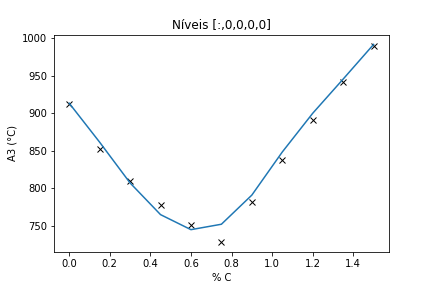
\includegraphics[width=.5\textwidth]{img/C0.png}}
\subfloat[\label{fig:C2}]{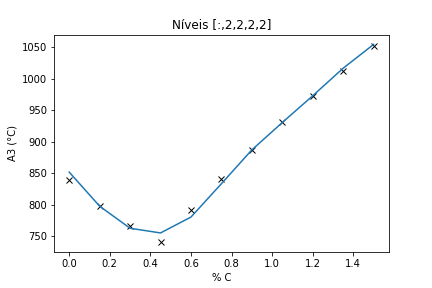
\includegraphics[width=.5\textwidth]{img/C2.png}}
\caption{Isopletas de Carbono geradas pelas predições da rede neural para (a) Nível 0; (b) Nível 2 }
\label{fig:C_NN_isop}
\end{figure}

\begin{figure}
\subfloat[\label{fig:Mn0}]{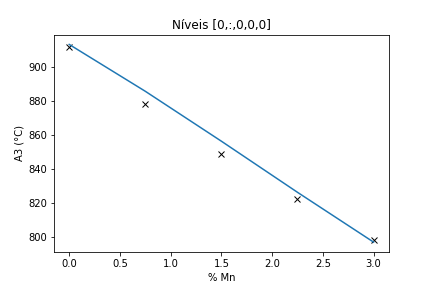
\includegraphics[width=.5\textwidth]{img/Mn0.png}}
\subfloat[\label{fig:Mn2}]{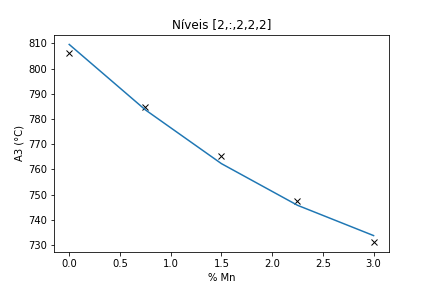
\includegraphics[width=.5\textwidth]{img/Mn2.png}}
\caption{Isopletas de Manganês geradas pelas predições da rede neural para (a) Nível 0; (b) Nível 2 }
\label{fig:Mn_NN_isop}
\end{figure}

\begin{figure}
\subfloat[\label{fig:Si0}]{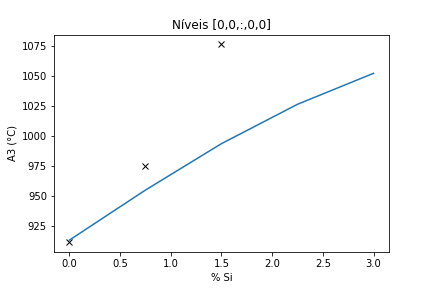
\includegraphics[width=.5\textwidth]{img/Si0.png}}
\subfloat[\label{fig:Si2}]{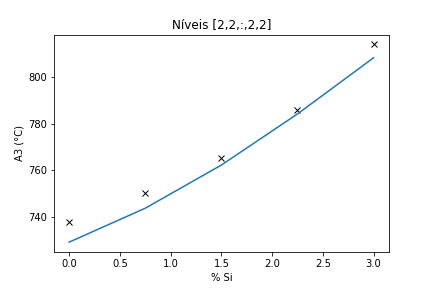
\includegraphics[width=.5\textwidth]{img/Si2.png}}
\caption{Isopletas de Silício geradas pelas predições da rede neural para (a) Nível 0; (b) Nível 2 }
\label{fig:Si_NN_isop}
\end{figure}

\begin{figure}
\subfloat[\label{fig:Cr0}]{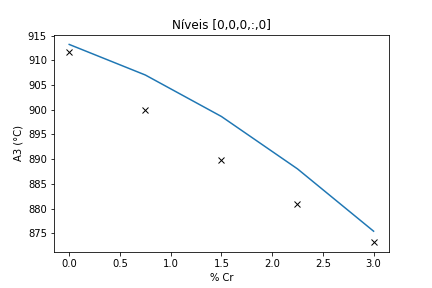
\includegraphics[width=.5\textwidth]{img/Cr0.png}}
\subfloat[\label{fig:Cr2}]{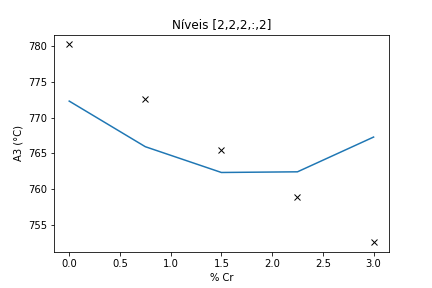
\includegraphics[width=.5\textwidth]{img/Cr2.png}}
\caption{Isopletas de Cromo geradas pelas predições da rede neural para (a) Nível 0; (b) Nível 2 }
\label{fig:Cr_NN_isop}
\end{figure}

\begin{figure}
\subfloat[\label{fig:Ni0}]{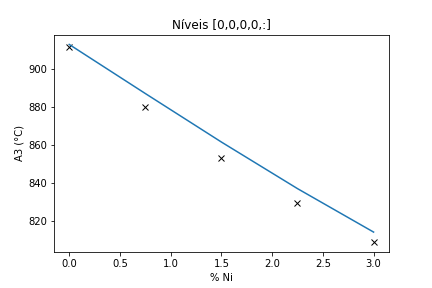
\includegraphics[width=.5\textwidth]{img/Ni0.png}}
\subfloat[\label{fig:Ni2}]{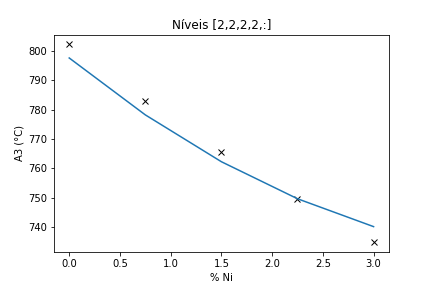
\includegraphics[width=.5\textwidth]{img/Ni2.png}}
\caption{Isopletas de Níquel geradas pelas predições da rede neural para (a) Nível 0; (b) Nível 2 }
\label{fig:Ni_NN_isop}
\end{figure}

Nota-se que, para a maioria dos casos, os valores preditos (linha cheia) são satisfatórios em relação ao esperado (pontos em forma de ``x'') .

Para o Carbono, a dificuldade está no ajuste do ponto de inversão da curva, ponto mais suscetível a erros, como foi observado na Figura \ref{fig:LR_A3} da regressão linear e na Figura \ref{fig:predict6} da predição da rede neural, na qual possivelmente os dados que destoam da reta estão próximos a esse ponto. Um conjunto de dados de treino com mais pontos corretos dessa região poderia contribuir para uma melhor predição.

Para baixas concentrações dos elementos, o modelo para o silício foi destoante, como mostra a Figura \ref{fig:Si0}. Uma possível explicação está no diagrama binário Fe-Si, da Figura \ref{fig:bin_fe-si}, que mostra o campo $\gamma$ fechado a baixas concentrações de Si. O mesmo vale para o cromo, que além de ser do grupo de domínio $\gamma$ fechado, tem um $\gamma$-\textit{loop}. Isso pode ter contribuído para uma má predição do modelo nesses casos.
% ARRUMAR: não sei muito bem o que dizer aqui

Apesar de o modelo não ter predito tão bem a influência de alguns elementos em A3, suas métricas foram consideradas satisfatórias. Para o ponto ótimo discutido anteriormente, de taxa de aprendizado 0.001, seis neurônios na camada intermediária e 100 iterações, o erro quadrático médio final foi de 0.0051 e o coeficiente de determinação ($R^{2}$), 0.9734.

\section{Comparação dos Modelos}

Com o propósito de comparar os modelos de regressão linear com o de rede neural para predição de A3, foi calculado o Coeficiente de Determinação de cada um deles, que pode ser visto na Tabela \ref{tab:r2_comparacao} a seguir.

\begin{table}
  \caption{Valores de $R^{2}$ para regressão linear e rede neural de A3}

  \begin{tabular}{ll}
  \hline
  Modelo                          & $R^{2}$ \\
  \hline
  Regressão Linear Hipoeutetóide  & 0.9607  \\
  Regressão Linear Hipereutetóide & 0.9971  \\
  Regressão Linear Total          & 0.8774  \\
  Rede Neural Artificial          & 0.9734  \\
  \hline
  \end{tabular}

  \label{tab:r2_comparacao}
\end{table}

É possível constatar que a regressão linear para os hipereutetóides foi o modelo com melhor ajuste, seguido pela rede neural e pela regressão linear hipoeutetóide. A regressão linear total foi a de menor ajuste, pois como discutido anteriormente, o ponto de inversão da curva não é bem predito.

O valor alto de $R^{2}$ para a rede neural torna menos provável a hipótese de a regressão linear apresentar overfit devido a parâmetros em excesso.

(\textit{A melhorar: inserir gráficos de valores preditos para Regressão Linear x Equação Empírica e Rede Neural x Equação Empírica})

\chapter{Conclusões}

Foi estudada a implementação de dois algoritmos de aprendizado de máquina para prever temperaturas críticas de transformações de fase em aços comuns de engenharia. Para isso, foi criado um banco de dados a partir de simulações termodinâmicas e algoritmos para extração dessas temperaturas críticas. Os dados foram analisados mediante comparação com equações empíricas e foram tratados antes de serem usados para o treino.

O modelo de regressão linear mostrou métricas bastante satisfatórias para a maior parte dos casos estudados, mesmo quando testado por um banco de dados aleatório. Sua desvantagem foi a necessidade de separação dos dados entre hipo e hipereutetóide para que o modelo tivesse melhor qualidade de predição. Ainda não foi descartada a hipótese de overfit e para tal deveriam ser estudadas outras métricas e realizar novos testes com outros bancos de dados.

A rede neural, por sua vez, foi capaz de prever a temperatura A3 sem a necessidade de separação pelo ponto eutetóide, apesar de não conseguir calcular tão bem as temperaturas próximas a esse ponto de inversão. Seu alto coeficiente de determinação diminui a probabilidade de o modelo de regressão estar com overfit causado por número de parâmetros em excesso.

\textit{(A melhorar: fazer comparação com métricas do trabalho de Gavard)}

\chapter{Sugestões para trabalhos futuros}

\textit{(Ainda será escrito. Envolverá os seguintes tópicos:)}

\begin{itemize}
\item Variar mais parâmetros da rede neural
\item Determinar carbono eutetóide: através de coeficientes das regressões lineares ou regressão logística
\item Criar uma ferramenta de visualização e interação com o usuário
\item Extrapolar o modelo para outras faixas de composição
\end{itemize}

\bibliography{tcc}

% \anexo{Composição química de aços de engenharia}
% \label{an:composicao}
% ARRUMAR: se der, adicionar tabelas


\anexo{Diagramas binários}
\label{an:diag_bin}

\begin{figure}
  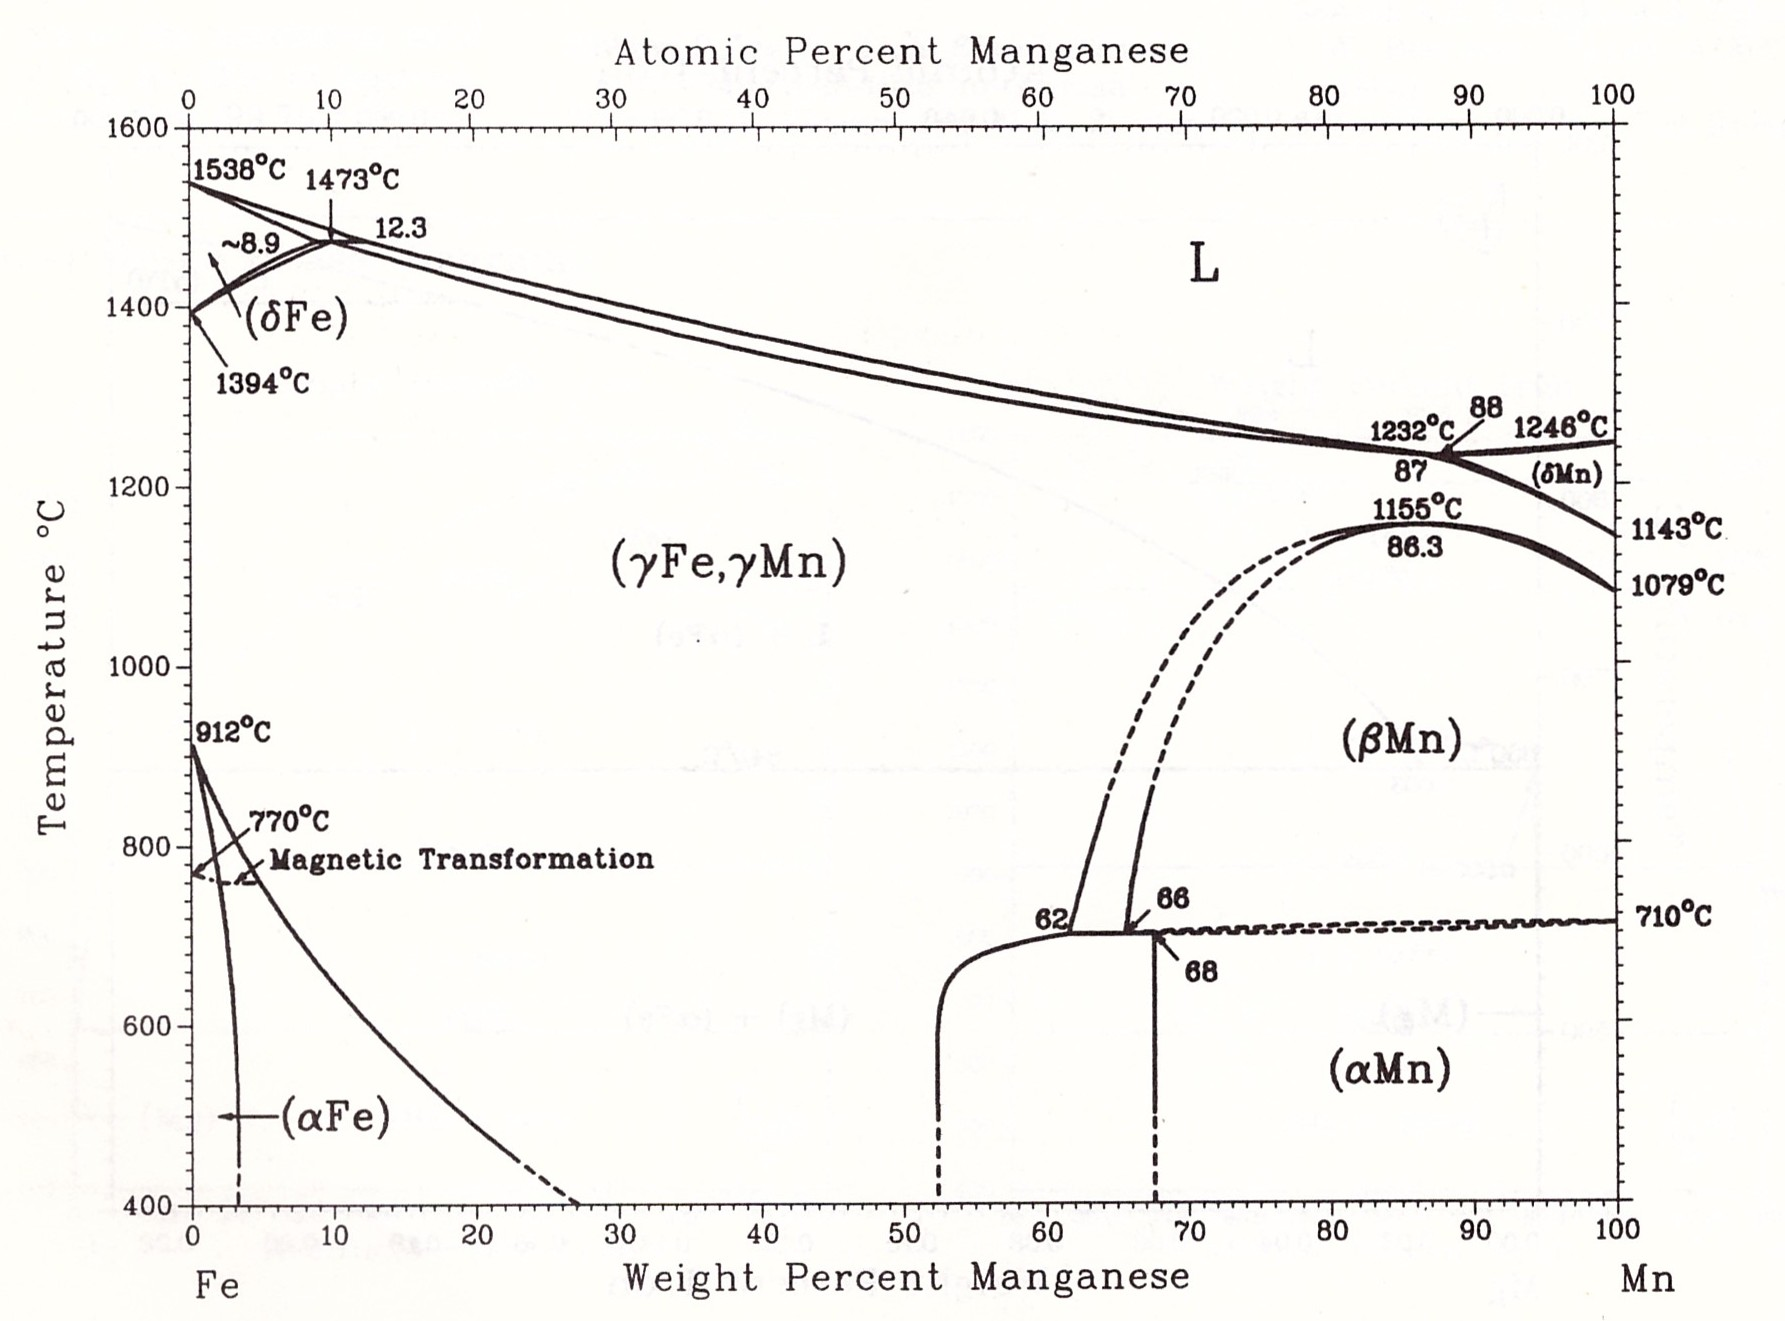
\includegraphics[width=1.1\textwidth]{img/Fe-Mn.jpg}
  \caption{Diagrama binário Fe-Mn}
  \label{fig:bin_fe-mn}
\end{figure}

\begin{figure}
  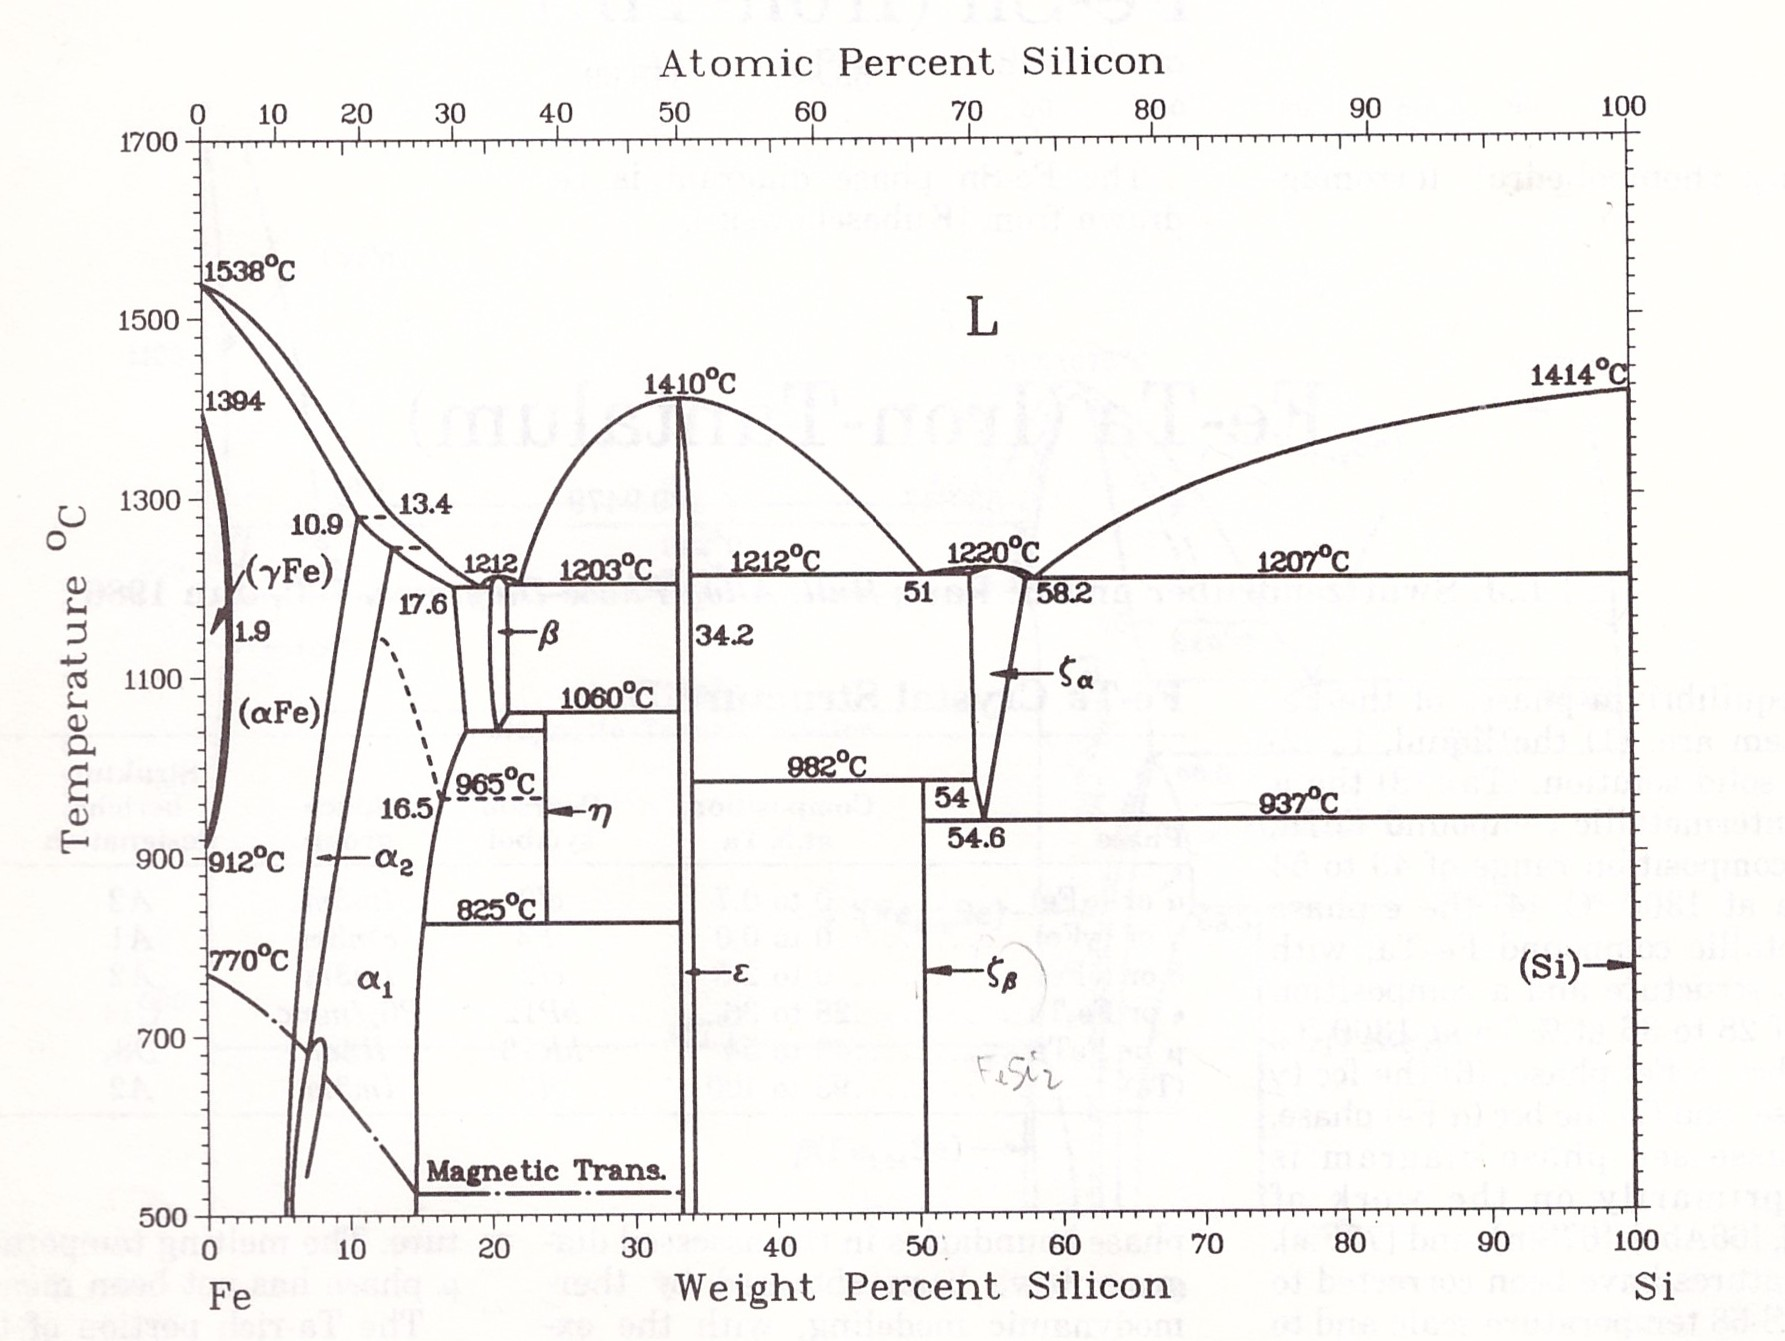
\includegraphics[width=1.1\textwidth]{img/Fe-Si.jpg}
  \caption{Diagrama binário Fe-Si}
  \label{fig:bin_fe-si}
\end{figure}

\begin{figure}
  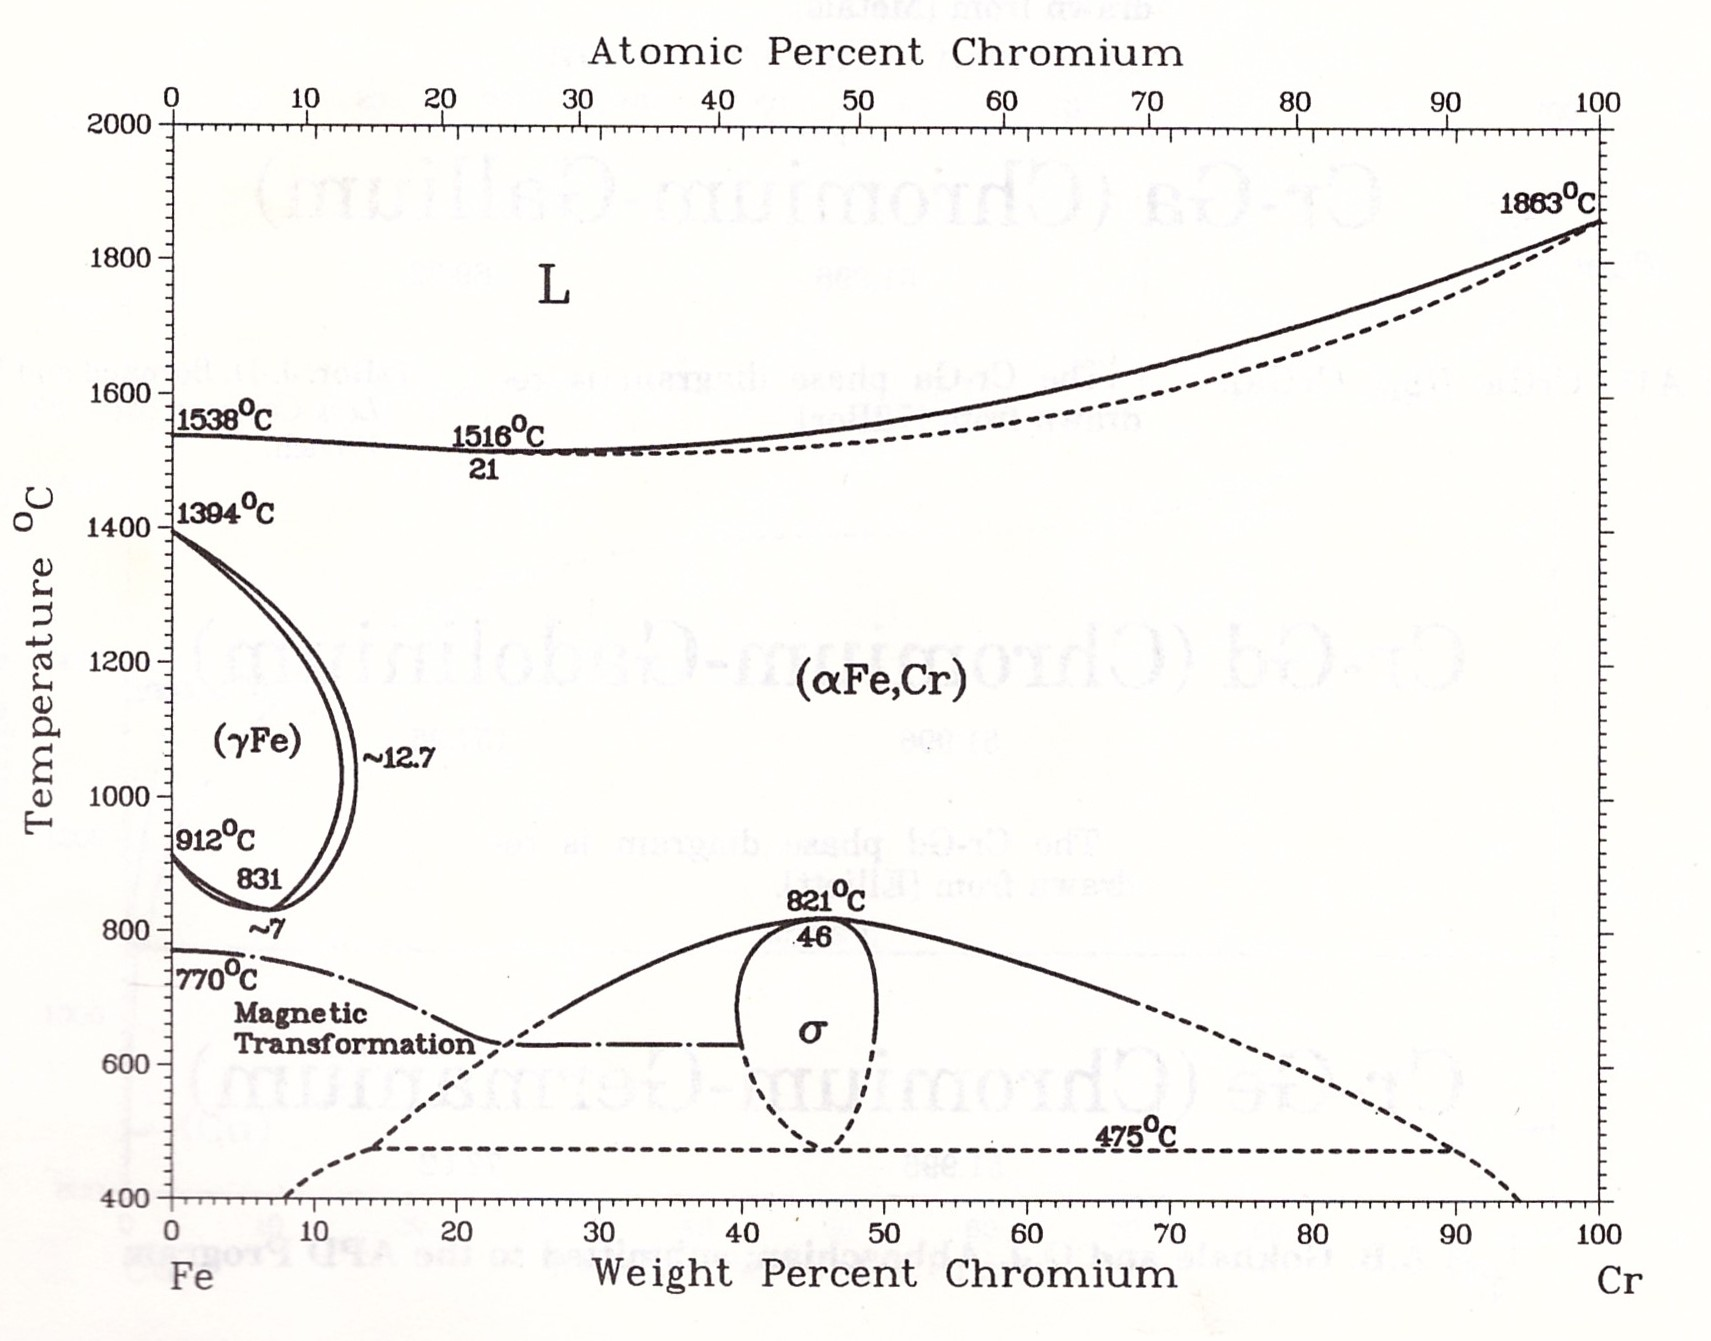
\includegraphics[width=1.1\textwidth]{img/Fe-Cr.jpg}
  \caption{Diagrama binário Fe-Cr}
  \label{fig:bin_fe-cr}
\end{figure}

\begin{figure}
  \includegraphics[width=1.1\textwidth]{img/Fe-Ni.jpg}
  \caption{Diagrama binário Fe-Ni}
  \label{fig:bin_fe-ni}
\end{figure}

\end{document}
